%%!!!!!!!!!!!!!!!!!!!!!!!!!!!!!!!!!!!!!!!!!!!!!!!!!!!!!!!!!!!!!!!!!!!!!!!!!!!!!!
%%%%%%%%%%%%%%%%%%%%%%%%%%%%%%%%%%%%%%%%%%%%%%%%%%%%%%%%%%%%%%%%%%%%%%%%%%%%%%%%
%% SECTION: Rozwiązanie techniczne
%%%%%%%%%%%%%%%%%%%%%%%%%%%%%%%%%%%%%%%%%%%%%%%%%%%%%%%%%%%%%%%%%%%%%%%%%%%%%%%%
%%!!!!!!!!!!!!!!!!!!!!!!!!!!!!!!!!!!!!!!!!!!!!!!!!!!!!!!!!!!!!!!!!!!!!!!!!!!!!!!
\section{Rozwiązanie techniczne}

%%%%%%%%%%%%%%%%%%%%%%%%%%%%%%%%%%%%%%%%%%%%%%%%%%%%%%%%%%%%%%%%%%%%%%%%%%%%%%%%
%% SUBSECTION: Zestaw uruchomieniowy P-NUCLEO-WB55
%%%%%%%%%%%%%%%%%%%%%%%%%%%%%%%%%%%%%%%%%%%%%%%%%%%%%%%%%%%%%%%%%%%%%%%%%%%%%%%%
\subsection{Zestaw uruchomieniowy P-NUCLEO-WB55}

\begin{figure}[!htb]
	\centering 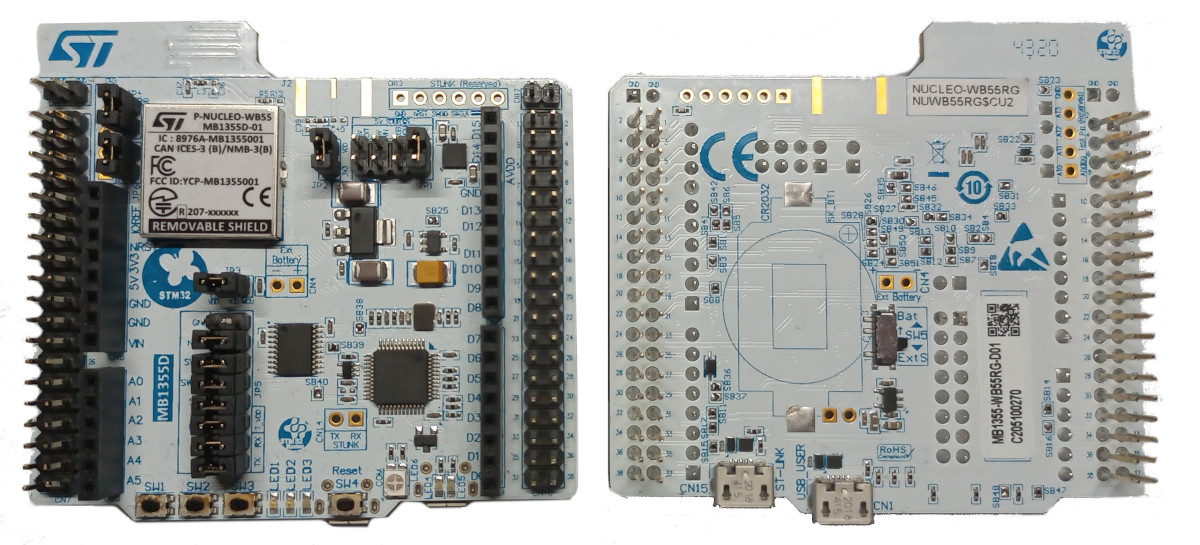
\includegraphics[width=0.618\linewidth]{nucleo_wb55.jpg}
	\caption{Zestaw uruchomieniowy P-NUCLEO-WB55. Źródło: \cite{noauthor_p-nucleo-wb55_nodate}}
	\label{rys:nucleo_wb55}
\end{figure}

%%%%%%%%%%%%%%%%%%%%%%%%%%%%%%%%%%%%%%%%%%%%%%%%%%%%%%%%%%%%%%%%%%%%%%%%%%%%%%%%
%% SUBSECTION: Zestaw pomiarowy X-NUCLEO-LPM01A
%%%%%%%%%%%%%%%%%%%%%%%%%%%%%%%%%%%%%%%%%%%%%%%%%%%%%%%%%%%%%%%%%%%%%%%%%%%%%%%%
\subsection{Zestaw pomiarowy X-NUCLEO-LPM01A}

\begin{figure}[!htb]
	\centering 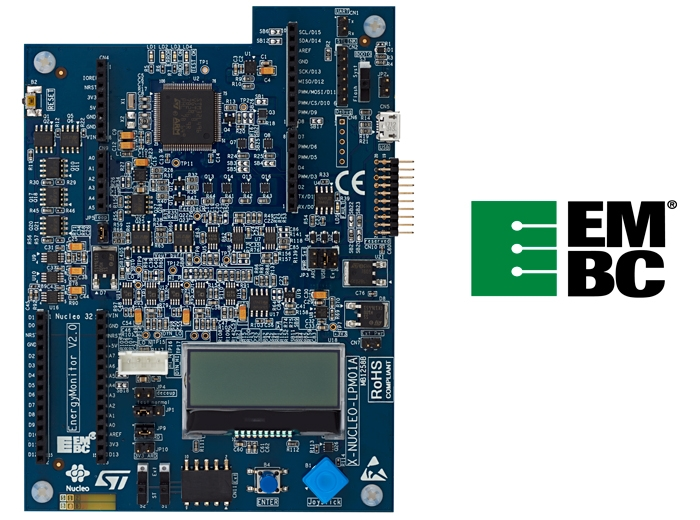
\includegraphics[width=0.618\linewidth]{st_power_measurement_unit.jpg}
	\caption{Zestaw pomiarowy X-NUCLEO-LPM01A. Źródło: \cite{noauthor_x-nucleo-lpm01a_nodate}}
	\label{rys:nucleo_lpm01a}
\end{figure}

%%%%%%%%%%%%%%%%%%%%%%%%%%%%%%%%%%%%%%%%%%%%%%%%%%%%%%%%%%%%%%%%%%%%%%%%%%%%%%%%
%% SUBSECTION: HAL i stos Bluetooth Low Energy
%%%%%%%%%%%%%%%%%%%%%%%%%%%%%%%%%%%%%%%%%%%%%%%%%%%%%%%%%%%%%%%%%%%%%%%%%%%%%%%%
\subsection{HAL i stos Bluetooth Low Energy}


%%!!!!!!!!!!!!!!!!!!!!!!!!!!!!!!!!!!!!!!!!!!!!!!!!!!!!!!!!!!!!!!!!!!!!!!!!!!!!!!
%%%%%%%%%%%%%%%%%%%%%%%%%%%%%%%%%%%%%%%%%%%%%%%%%%%%%%%%%%%%%%%%%%%%%%%%%%%%%%%%
%% SECTION: Przygotowanie eksperymentu
%%%%%%%%%%%%%%%%%%%%%%%%%%%%%%%%%%%%%%%%%%%%%%%%%%%%%%%%%%%%%%%%%%%%%%%%%%%%%%%%
%%!!!!!!!!!!!!!!!!!!!!!!!!!!!!!!!!!!!!!!!!!!!!!!!!!!!!!!!!!!!!!!!!!!!!!!!!!!!!!!
\section{Przygotowanie eksperymentu}

%%%%%%%%%%%%%%%%%%%%%%%%%%%%%%%%%%%%%%%%%%%%%%%%%%%%%%%%%%%%%%%%%%%%%%%%%%%%%%%%
%% SUBSECTION: Oprogramowanie mikrokontrolera
%%%%%%%%%%%%%%%%%%%%%%%%%%%%%%%%%%%%%%%%%%%%%%%%%%%%%%%%%%%%%%%%%%%%%%%%%%%%%%%%
\subsection{Oprogramowanie mikrokontrolera}

%%%%%%%%%%%%%%%%%%%%%%%%%%%%%%%%%%%%%%%%%%%%%%%%%%%%%%%%%%%%%%%%%%%%%%%%%%%%%%%%
%% SUBSECTION: Oprogramowanie PC
%%%%%%%%%%%%%%%%%%%%%%%%%%%%%%%%%%%%%%%%%%%%%%%%%%%%%%%%%%%%%%%%%%%%%%%%%%%%%%%%
\subsection{Oprogramowanie PC}

%%%%%%%%%%%%%%%%%%%%%%%%%%%%%%%%%%%%%%%%%%%%%%%%%%%%%%%%%%%%%%%%%%%%%%%%%%%%%%%%
%% SUBSECTION: Pozostały sprzęt
%%%%%%%%%%%%%%%%%%%%%%%%%%%%%%%%%%%%%%%%%%%%%%%%%%%%%%%%%%%%%%%%%%%%%%%%%%%%%%%%
\subsection{Pozostały sprzęt}


%%!!!!!!!!!!!!!!!!!!!!!!!!!!!!!!!!!!!!!!!!!!!!!!!!!!!!!!!!!!!!!!!!!!!!!!!!!!!!!!
%%%%%%%%%%%%%%%%%%%%%%%%%%%%%%%%%%%%%%%%%%%%%%%%%%%%%%%%%%%%%%%%%%%%%%%%%%%%%%%%
%% SECTION: Zużycie energii
%%%%%%%%%%%%%%%%%%%%%%%%%%%%%%%%%%%%%%%%%%%%%%%%%%%%%%%%%%%%%%%%%%%%%%%%%%%%%%%%
%%!!!!!!!!!!!!!!!!!!!!!!!!!!!!!!!!!!!!!!!!!!!!!!!!!!!!!!!!!!!!!!!!!!!!!!!!!!!!!!
\section{Zużycie energii}

%%%%%%%%%%%%%%%%%%%%%%%%%%%%%%%%%%%%%%%%%%%%%%%%%%%%%%%%%%%%%%%%%%%%%%%%%%%%%%%%
%% SUBSECTION: Metodologia badania
%%%%%%%%%%%%%%%%%%%%%%%%%%%%%%%%%%%%%%%%%%%%%%%%%%%%%%%%%%%%%%%%%%%%%%%%%%%%%%%%
\subsection{Metodologia badania}

%%%%%%%%%%%%%%%%%%%%%%%%%%%%%%%%%%%%%%%%%%%%%%%%%%%%%%%%%%%%%%%%%%%%%%%%%%%%%%%%
%% SUBSECTION: BT Low Energy - Usługa Heart Rate
%%%%%%%%%%%%%%%%%%%%%%%%%%%%%%%%%%%%%%%%%%%%%%%%%%%%%%%%%%%%%%%%%%%%%%%%%%%%%%%%
\subsection{BT Low Energy - Usługa Heart Rate}

\begin{figure}[!htb]
	\centering 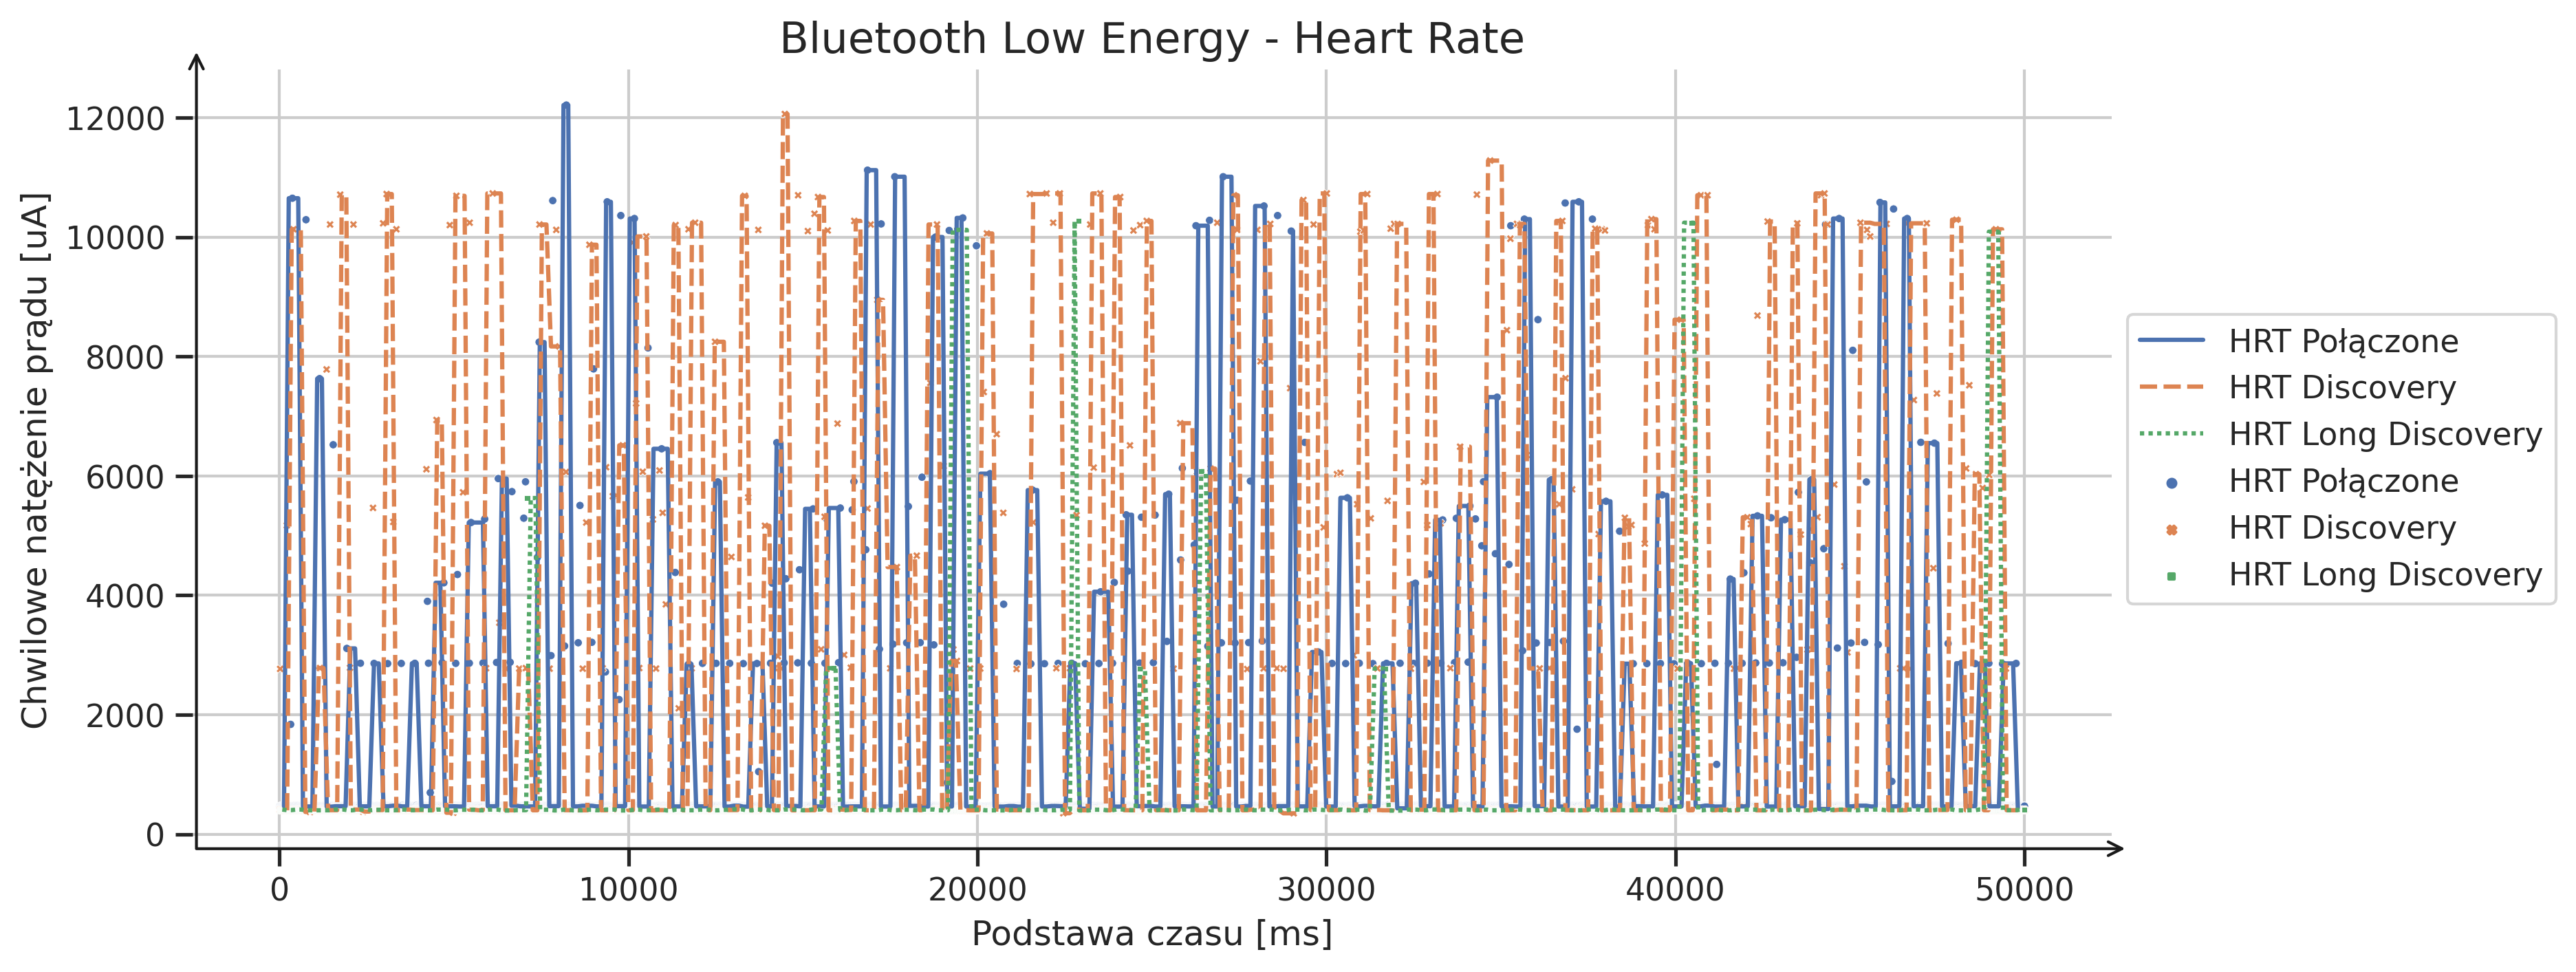
\includegraphics[width=0.99\linewidth]{power_ble_hr_amps.png}
	\caption{Charakterystyka czasowa poboru prądu dla BLE i usługi Heart Rate}
	\label{rys:power_ble_hr_amps}
\end{figure}

\begin{figure}[!htb]
	\centering 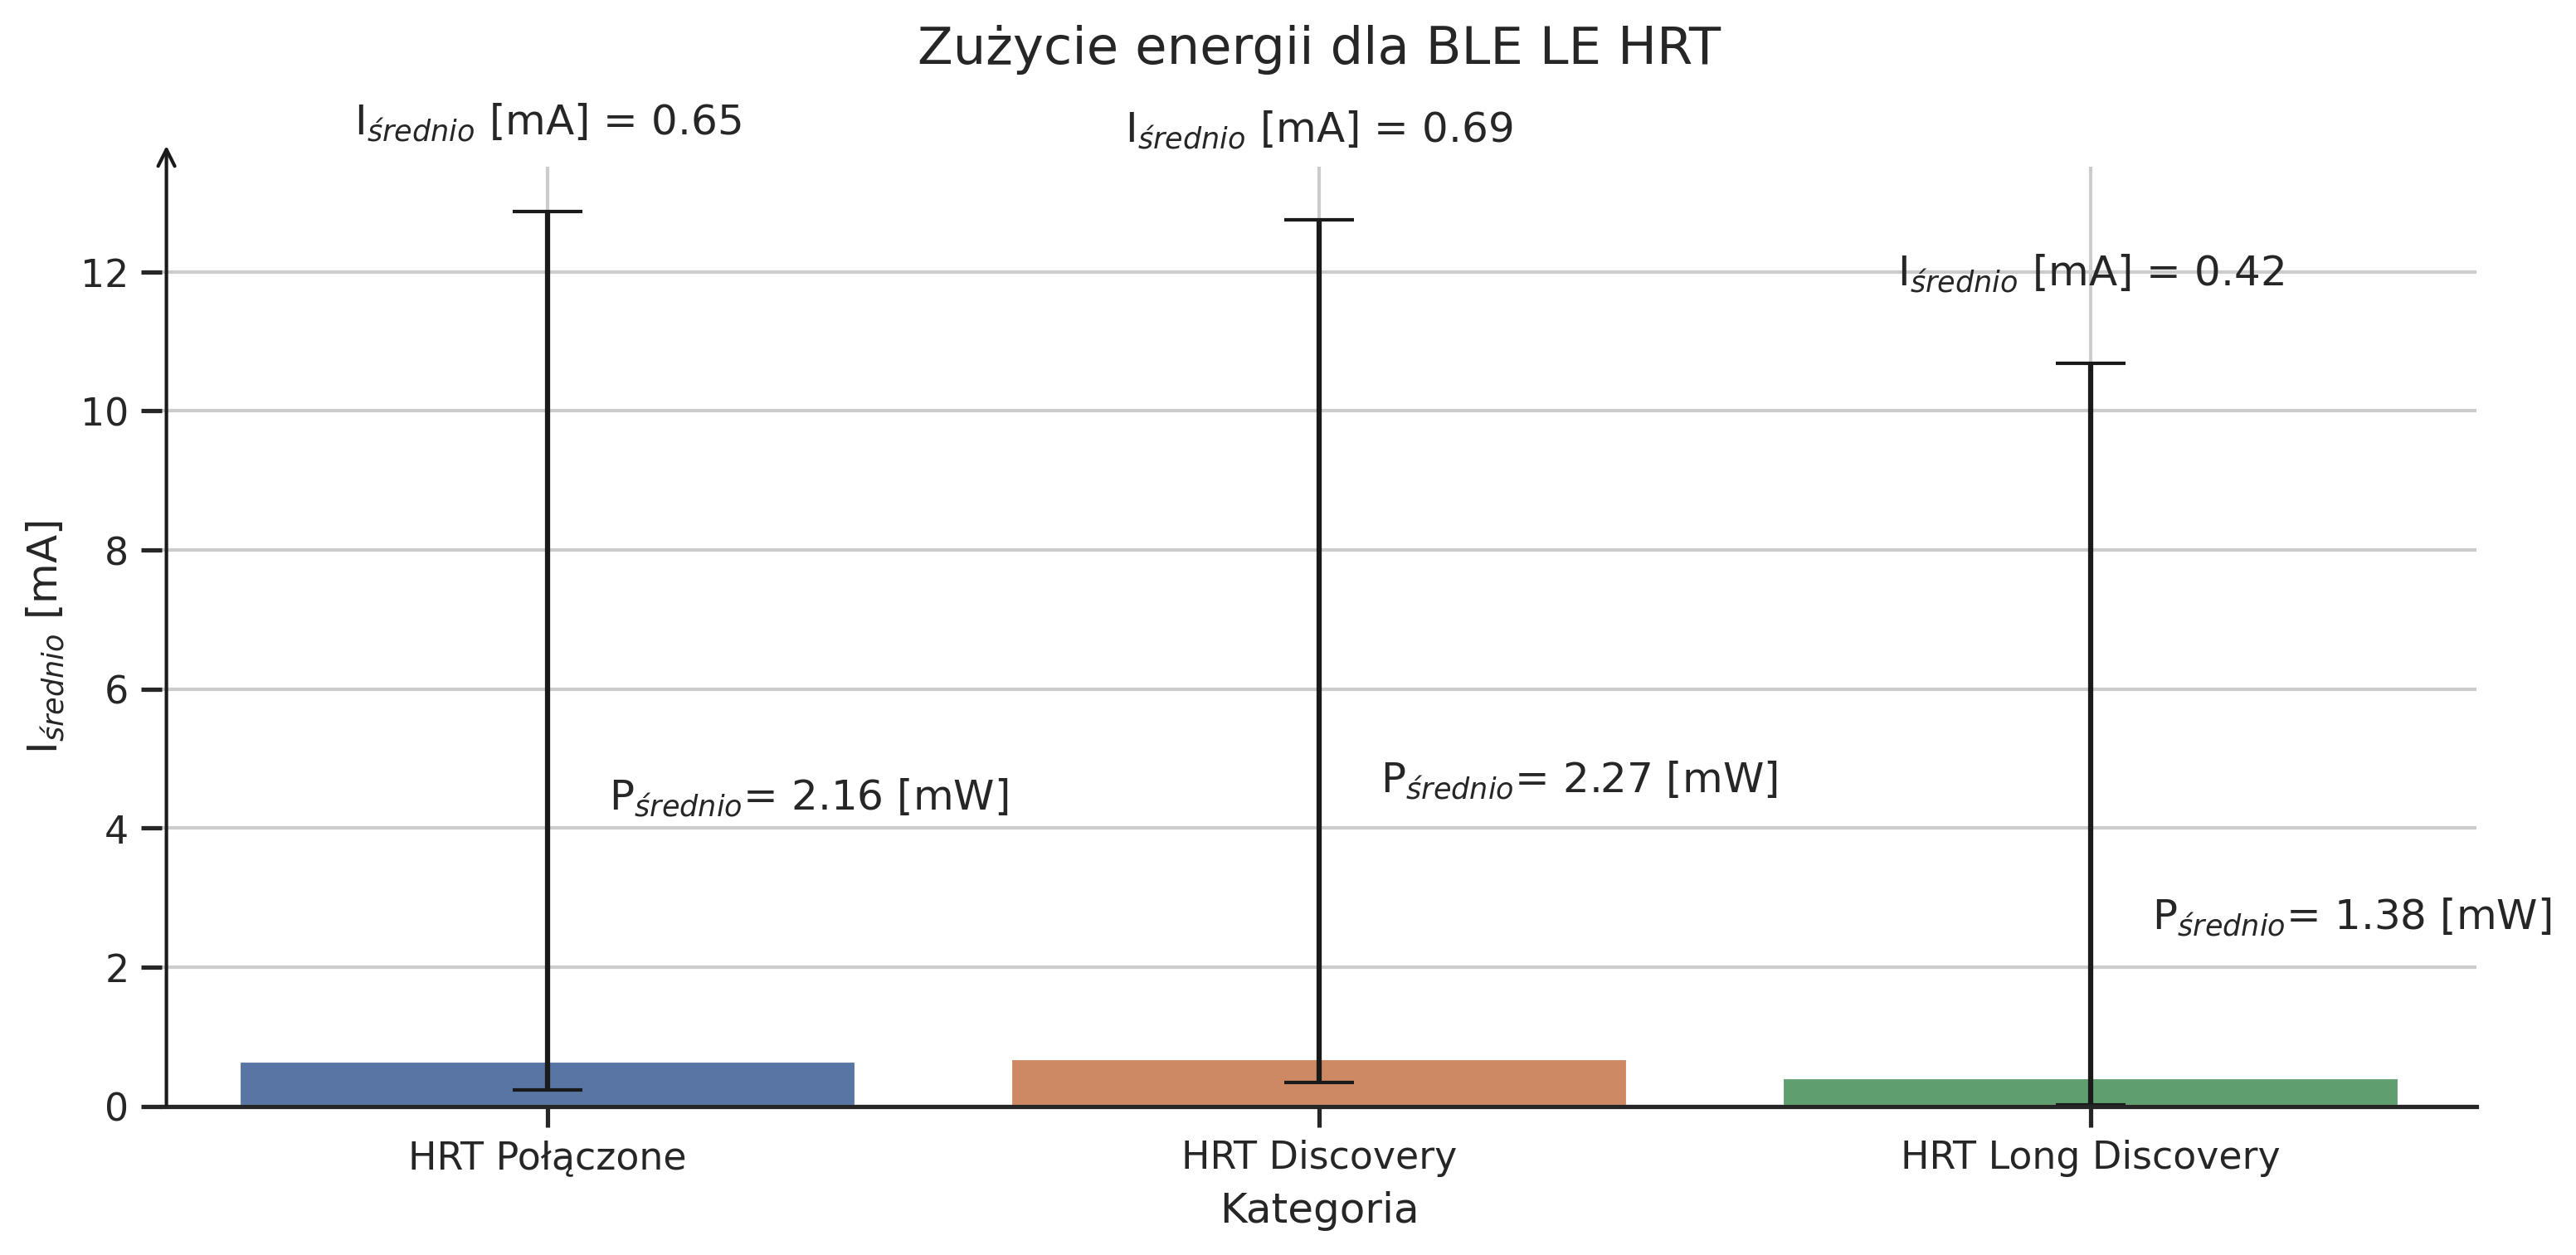
\includegraphics[width=0.99\linewidth]{power_ble_hr_amps_usage_juxtaposition.png}
	\caption{Zestawienie zużycia prądu dla usługi Heart Rate w zależności od trybu działania}
	\label{rys:power_ble_hr_amps_usage_juxtaposition}
\end{figure}

%%%%%%%%%%%%%%%%%%%%%%%%%%%%%%%%%%%%%%%%%%%%%%%%%%%%%%%%%%%%%%%%%%%%%%%%%%%%%%%%
%% SUBSECTION: BLE Mesh - Model Generic OnOff
%%%%%%%%%%%%%%%%%%%%%%%%%%%%%%%%%%%%%%%%%%%%%%%%%%%%%%%%%%%%%%%%%%%%%%%%%%%%%%%%
\subsection{BLE Mesh - Model Generic OnOff}

Pomiary dla BLE Mesh uwzględniające dwa tryby działania: sieć w oczekująca na komunikaty oraz podczas działania aktywnego korzystania z Modelu Generic OnOff.

\begin{figure}[!htb]
	\centering 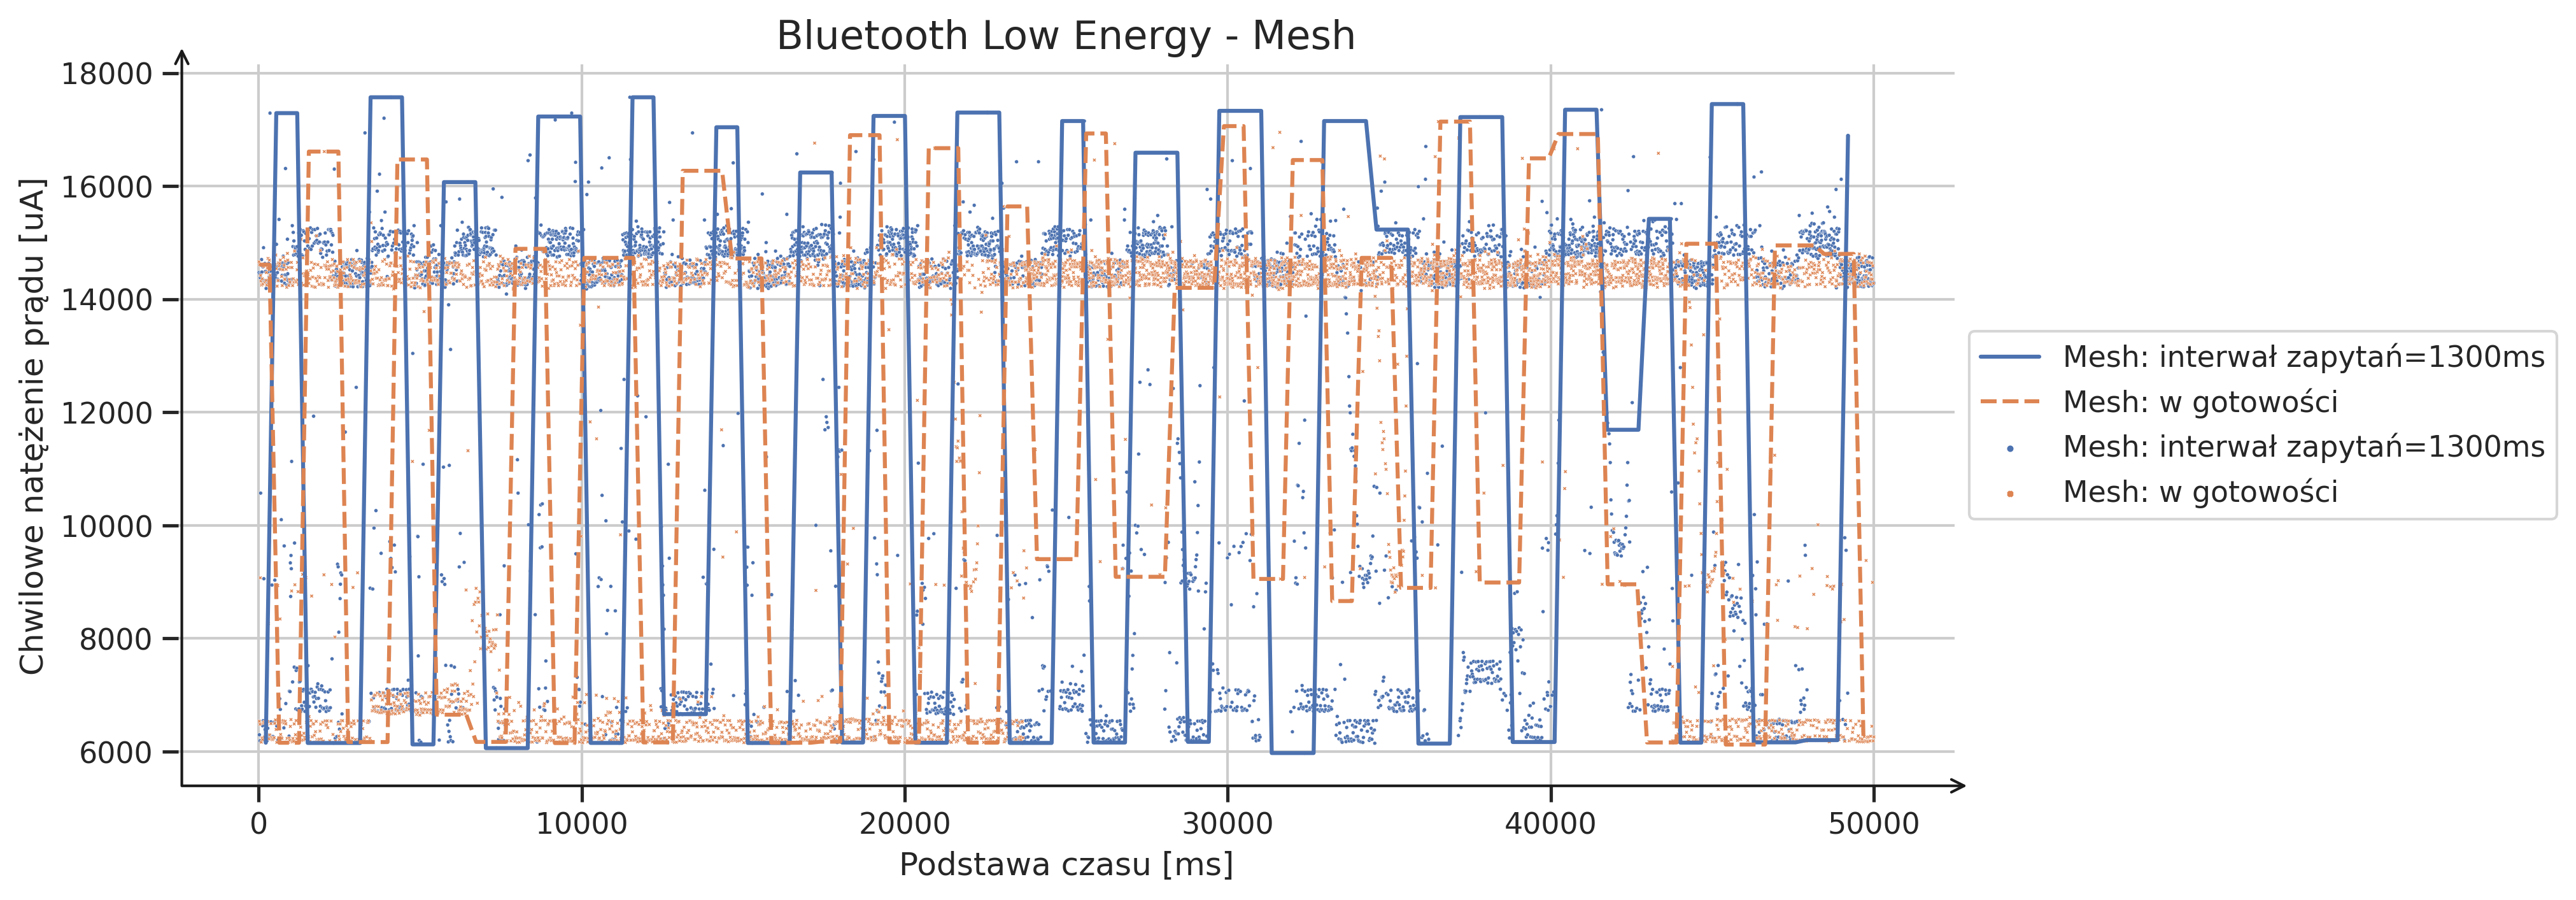
\includegraphics[width=0.99\linewidth]{power_ble_mesh_amps.png} 
	\caption{Charakterystyka czasowa poboru prądu dla BLE Mesh i modelu Generic OnOff}
	\label{rys:power_ble_mesh_amps}
\end{figure}

\begin{figure}[!htb]
	\centering 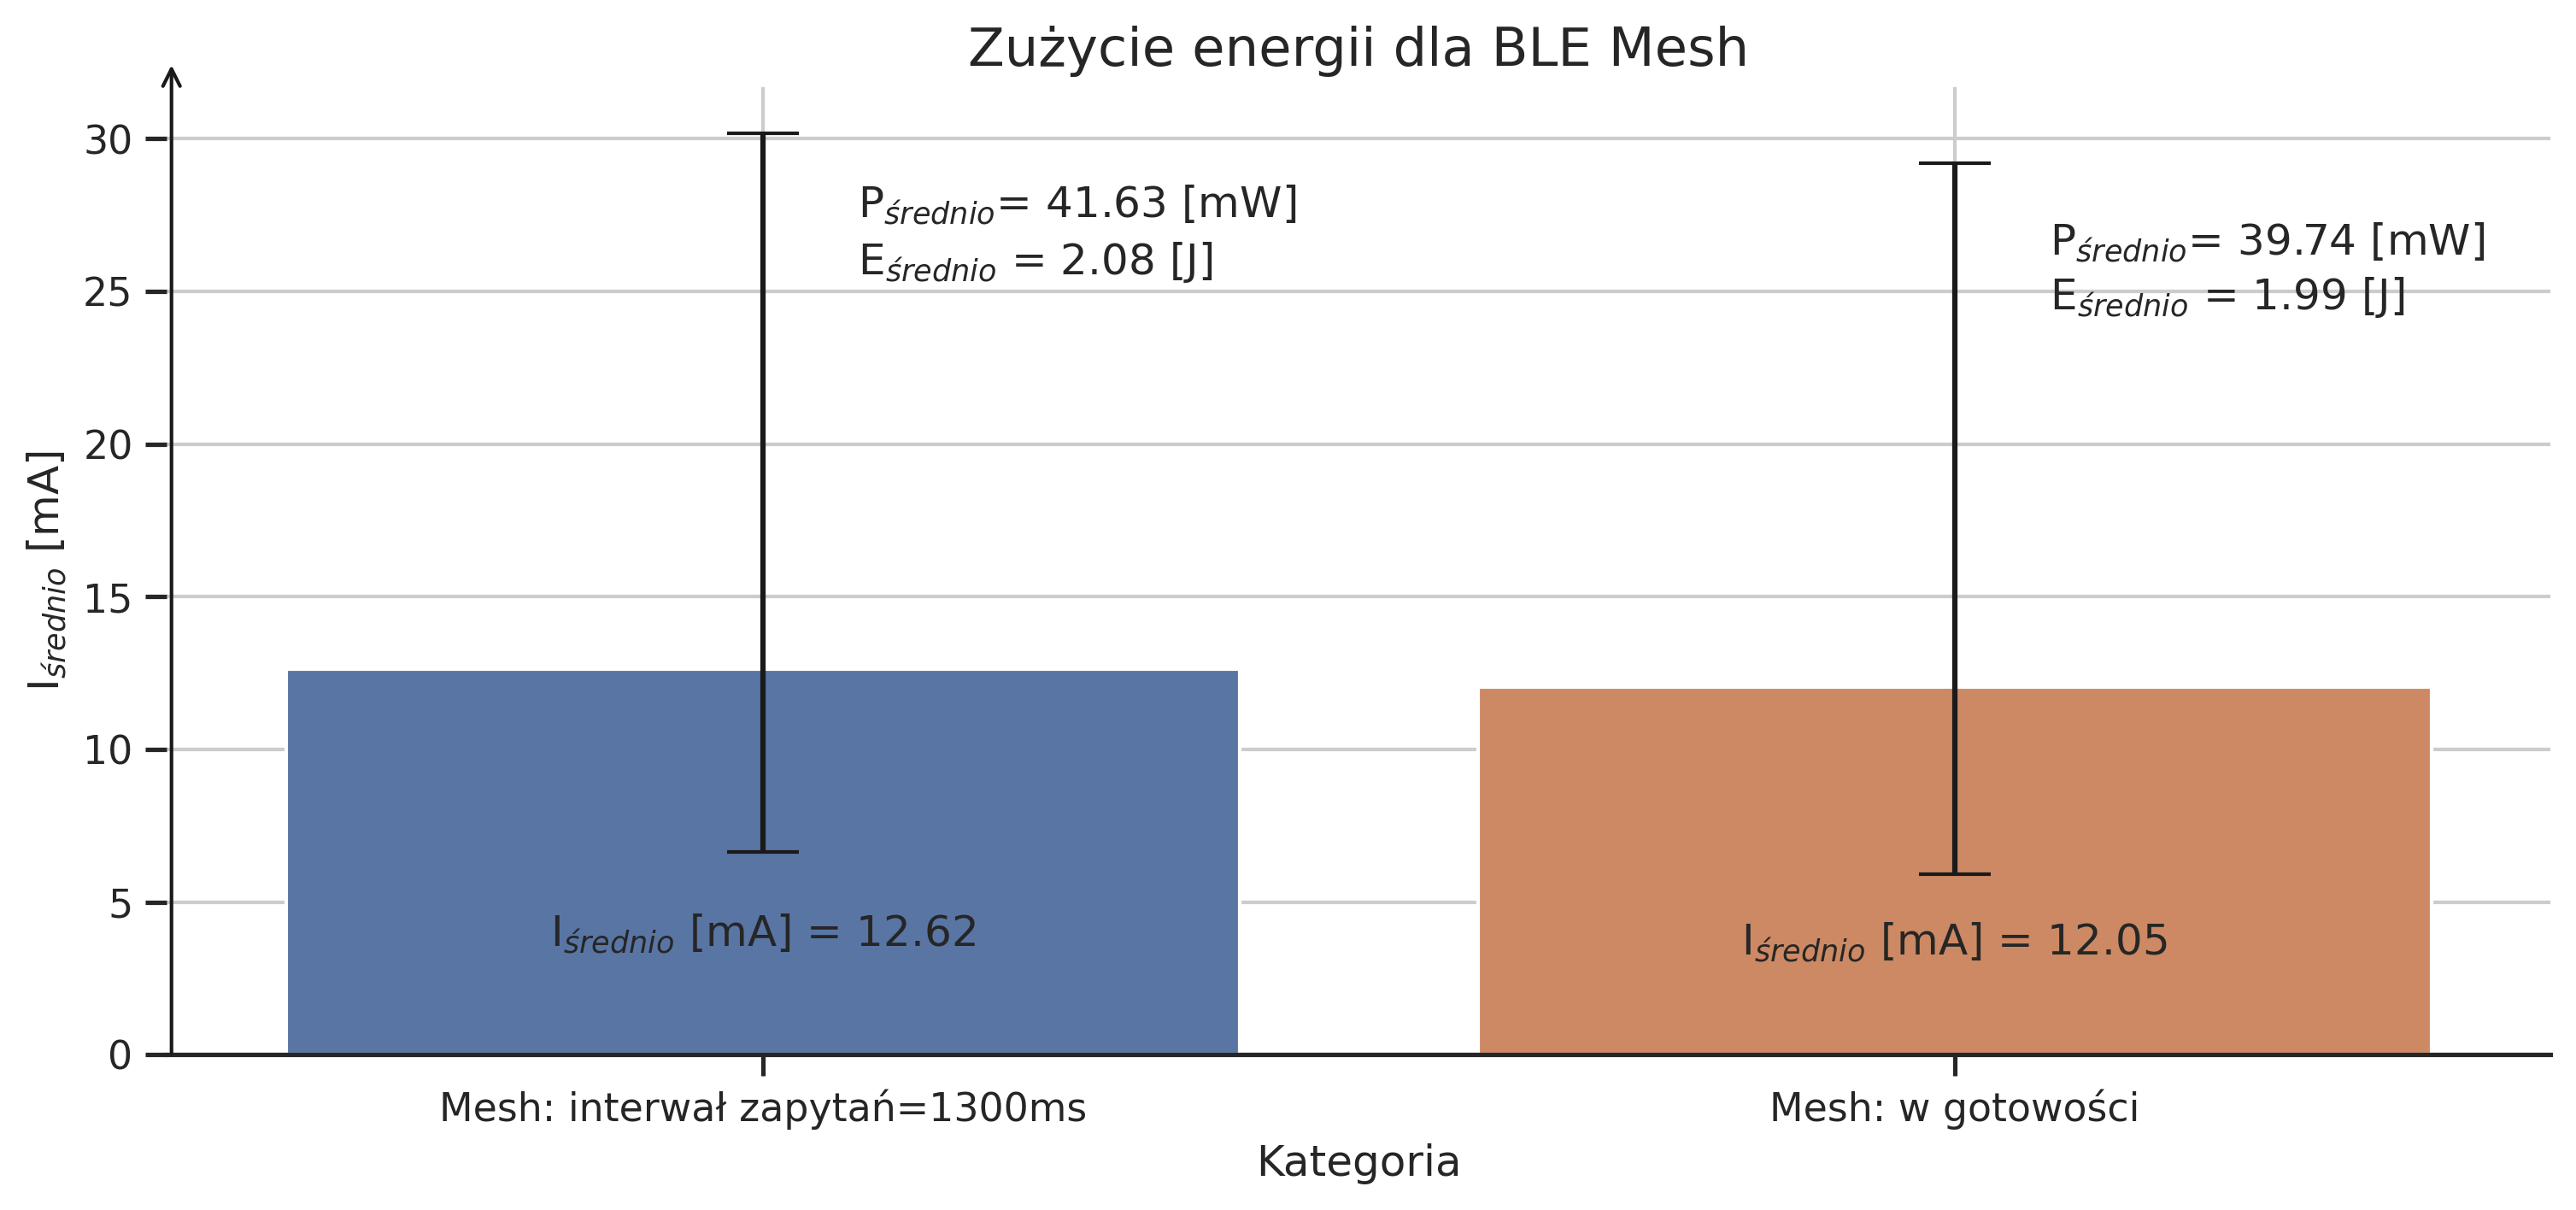
\includegraphics[width=0.99\linewidth]{power_ble_mesh_amps_usage_juxtaposition.png} 
	\caption{Zestawienie zużycia prądu dla BLE Mesh w zależności od trybu działania}
	\label{rys:power_ble_mesh_amps_usage_juxtaposition}
\end{figure}

\begin{figure}[!htb]
	\centering 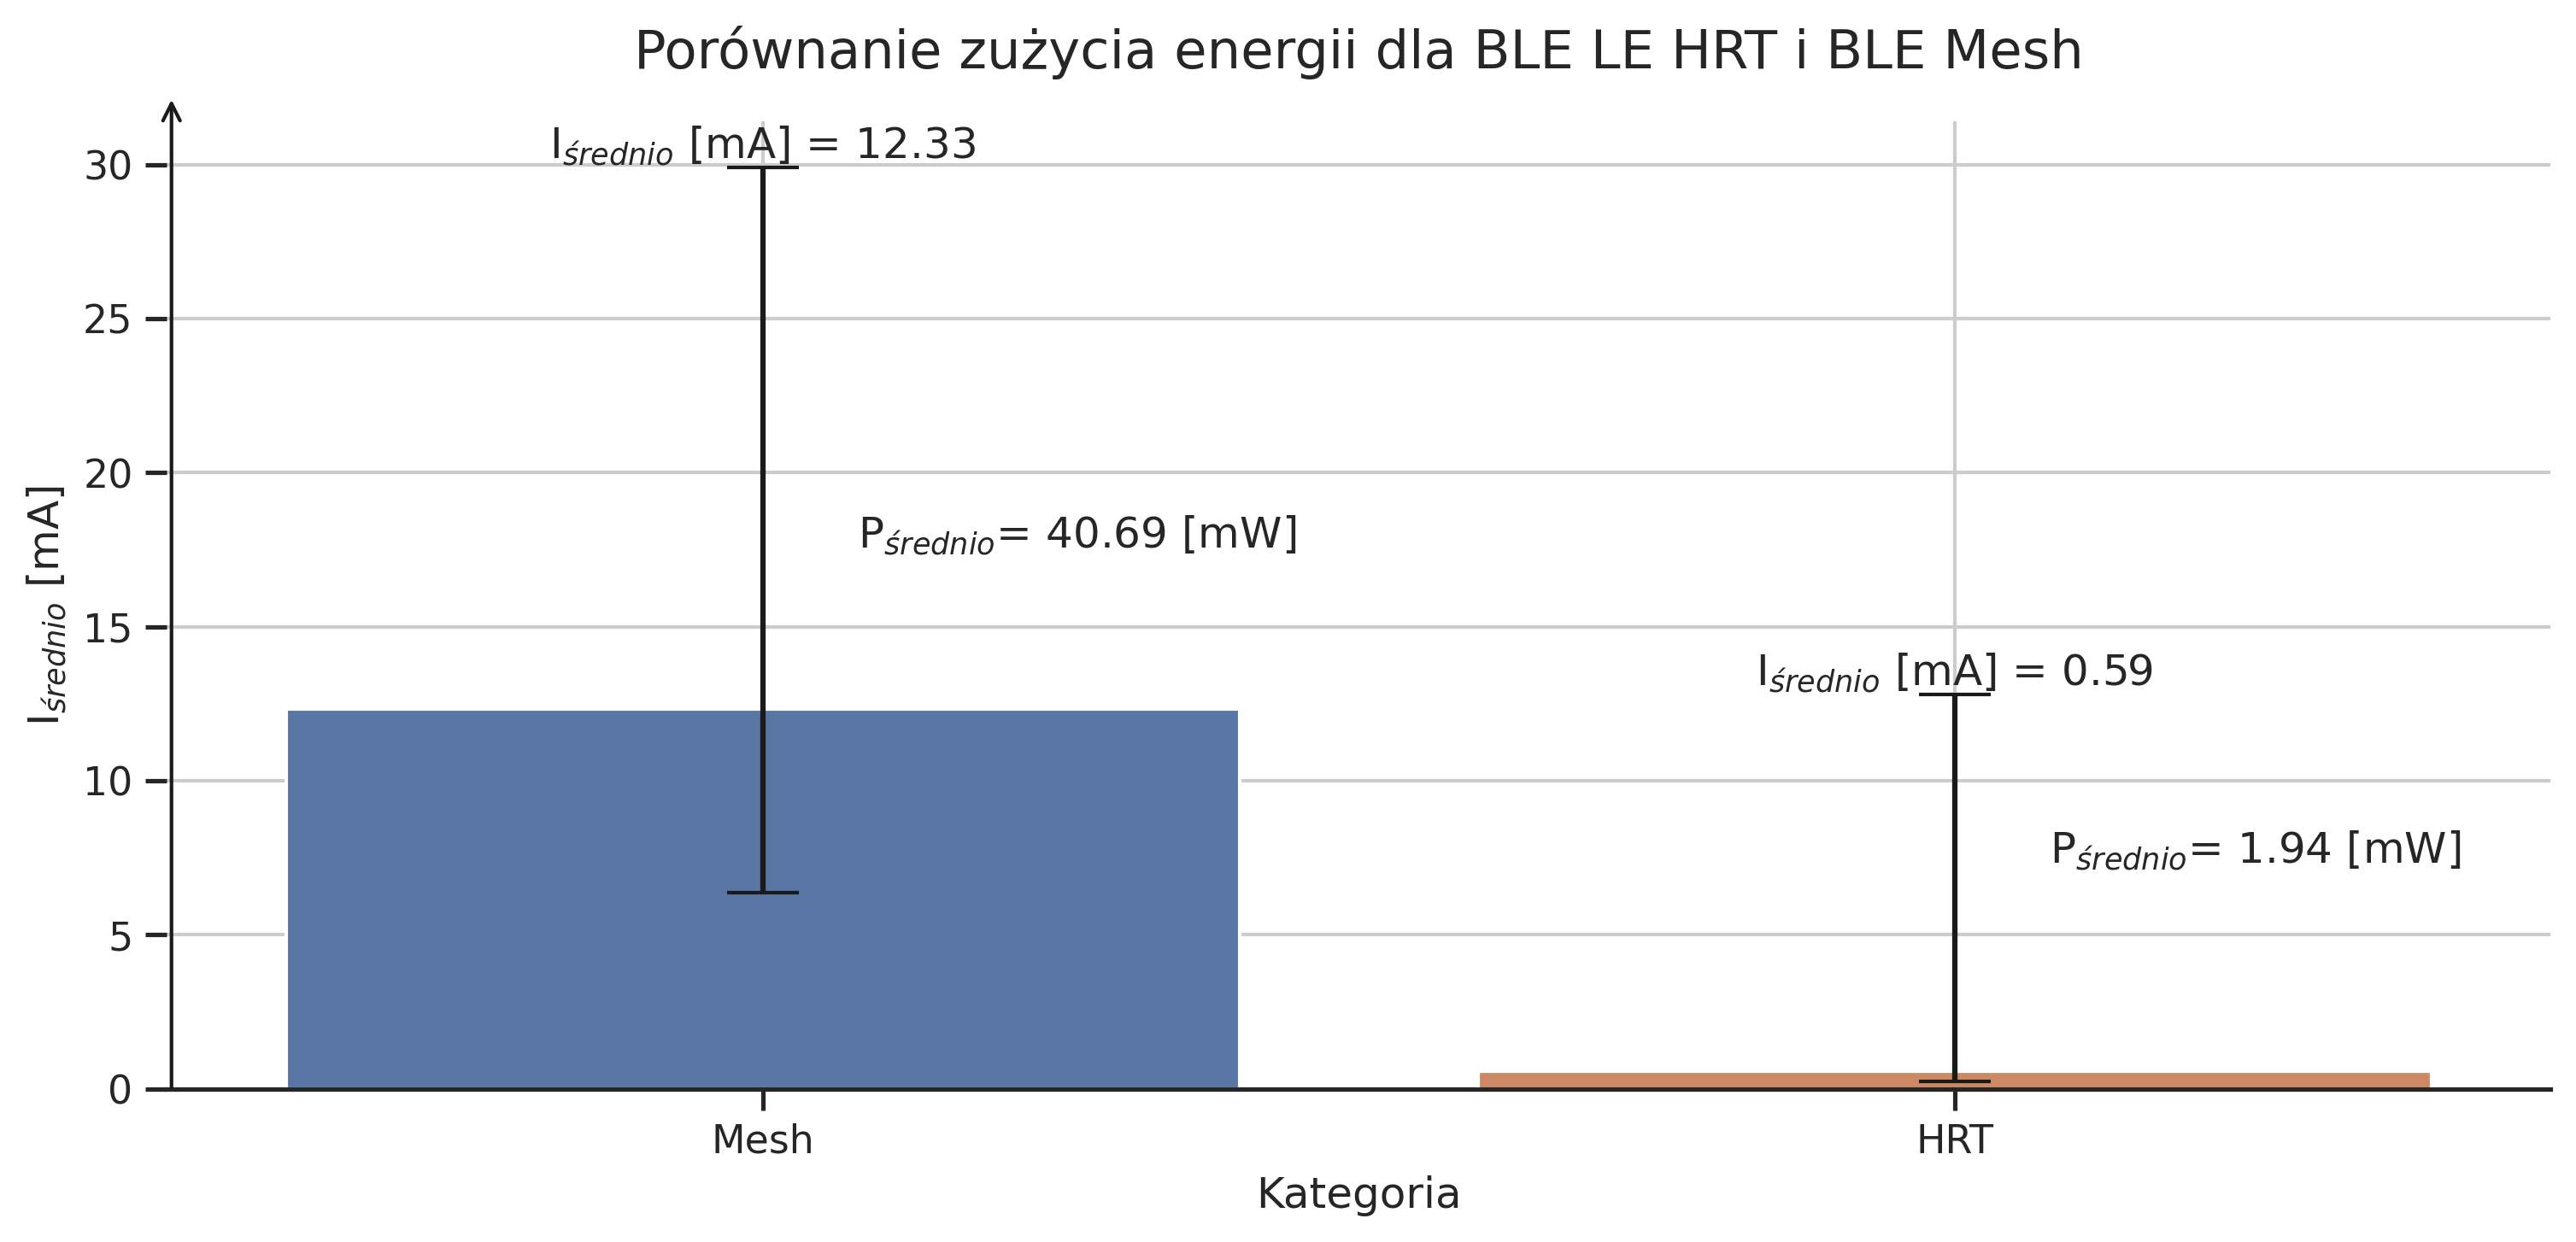
\includegraphics[width=0.99\linewidth]{power_ble_consumption_comparison.png} 
	\caption{Porównanie średniego zużycia energii pomiędzy BT Low Energy HRT i BLE Mesh}
	\label{rys:power_ble_consumption_comparison}
\end{figure}



%%!!!!!!!!!!!!!!!!!!!!!!!!!!!!!!!!!!!!!!!!!!!!!!!!!!!!!!!!!!!!!!!!!!!!!!!!!!!!!!
%%%%%%%%%%%%%%%%%%%%%%%%%%%%%%%%%%%%%%%%%%%%%%%%%%%%%%%%%%%%%%%%%%%%%%%%%%%%%%%%
%% SECTION: Packet Error Rate
%%%%%%%%%%%%%%%%%%%%%%%%%%%%%%%%%%%%%%%%%%%%%%%%%%%%%%%%%%%%%%%%%%%%%%%%%%%%%%%%
%%!!!!!!!!!!!!!!!!!!!!!!!!!!!!!!!!!!!!!!!!!!!!!!!!!!!!!!!!!!!!!!!!!!!!!!!!!!!!!!
\section{Packet Error Rate}

%%%%%%%%%%%%%%%%%%%%%%%%%%%%%%%%%%%%%%%%%%%%%%%%%%%%%%%%%%%%%%%%%%%%%%%%%%%%%%%%
%% SUBSECTION: Zależność PER względem odległości między węzłami
%%%%%%%%%%%%%%%%%%%%%%%%%%%%%%%%%%%%%%%%%%%%%%%%%%%%%%%%%%%%%%%%%%%%%%%%%%%%%%%%
\subsection{Metodologia badania}

\begin{figure}[!htb]
	\centering 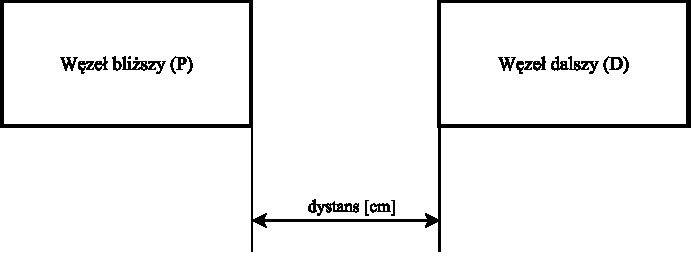
\includegraphics[width=0.618\linewidth]{per_two_nodes.pdf} 
	\caption{Dystans pomiędzy węzłami dla sieci dwóch mikrokontrolerów}
	\label{rys:two_nodes_setup}
\end{figure}

Rysunek ~\ref{rys:two_nodes_setup}

\begin{figure}[!htb]
	\centering 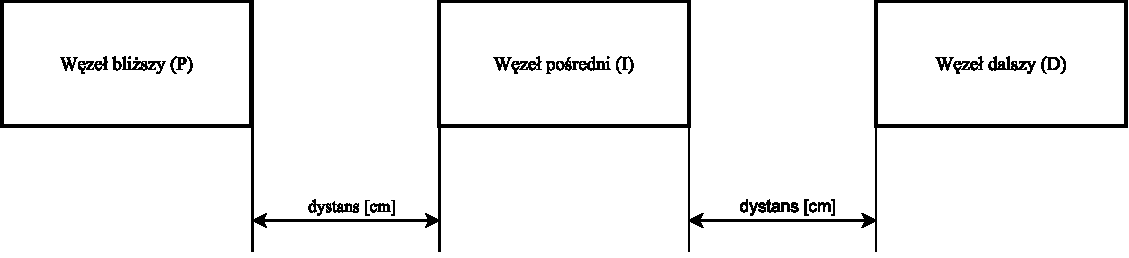
\includegraphics[width=0.99\linewidth]{per_three_nodes.pdf} 
	\caption{Dystans pomiędzy węzłami dla sieci trzech mikrokontrolerów}
	\label{rys:three_nodes_setup}
\end{figure}

%%%%%%%%%%%%%%%%%%%%%%%%%%%%%%%%%%%%%%%%%%%%%%%%%%%%%%%%%%%%%%%%%%%%%%%%%%%%%%%%
%% SUBSECTION: Zależność PER względem częstości zapytań
%%%%%%%%%%%%%%%%%%%%%%%%%%%%%%%%%%%%%%%%%%%%%%%%%%%%%%%%%%%%%%%%%%%%%%%%%%%%%%%%
\subsection{Zależność PER względem częstości zapytań}

\begin{figure}[!htb]
	\centering 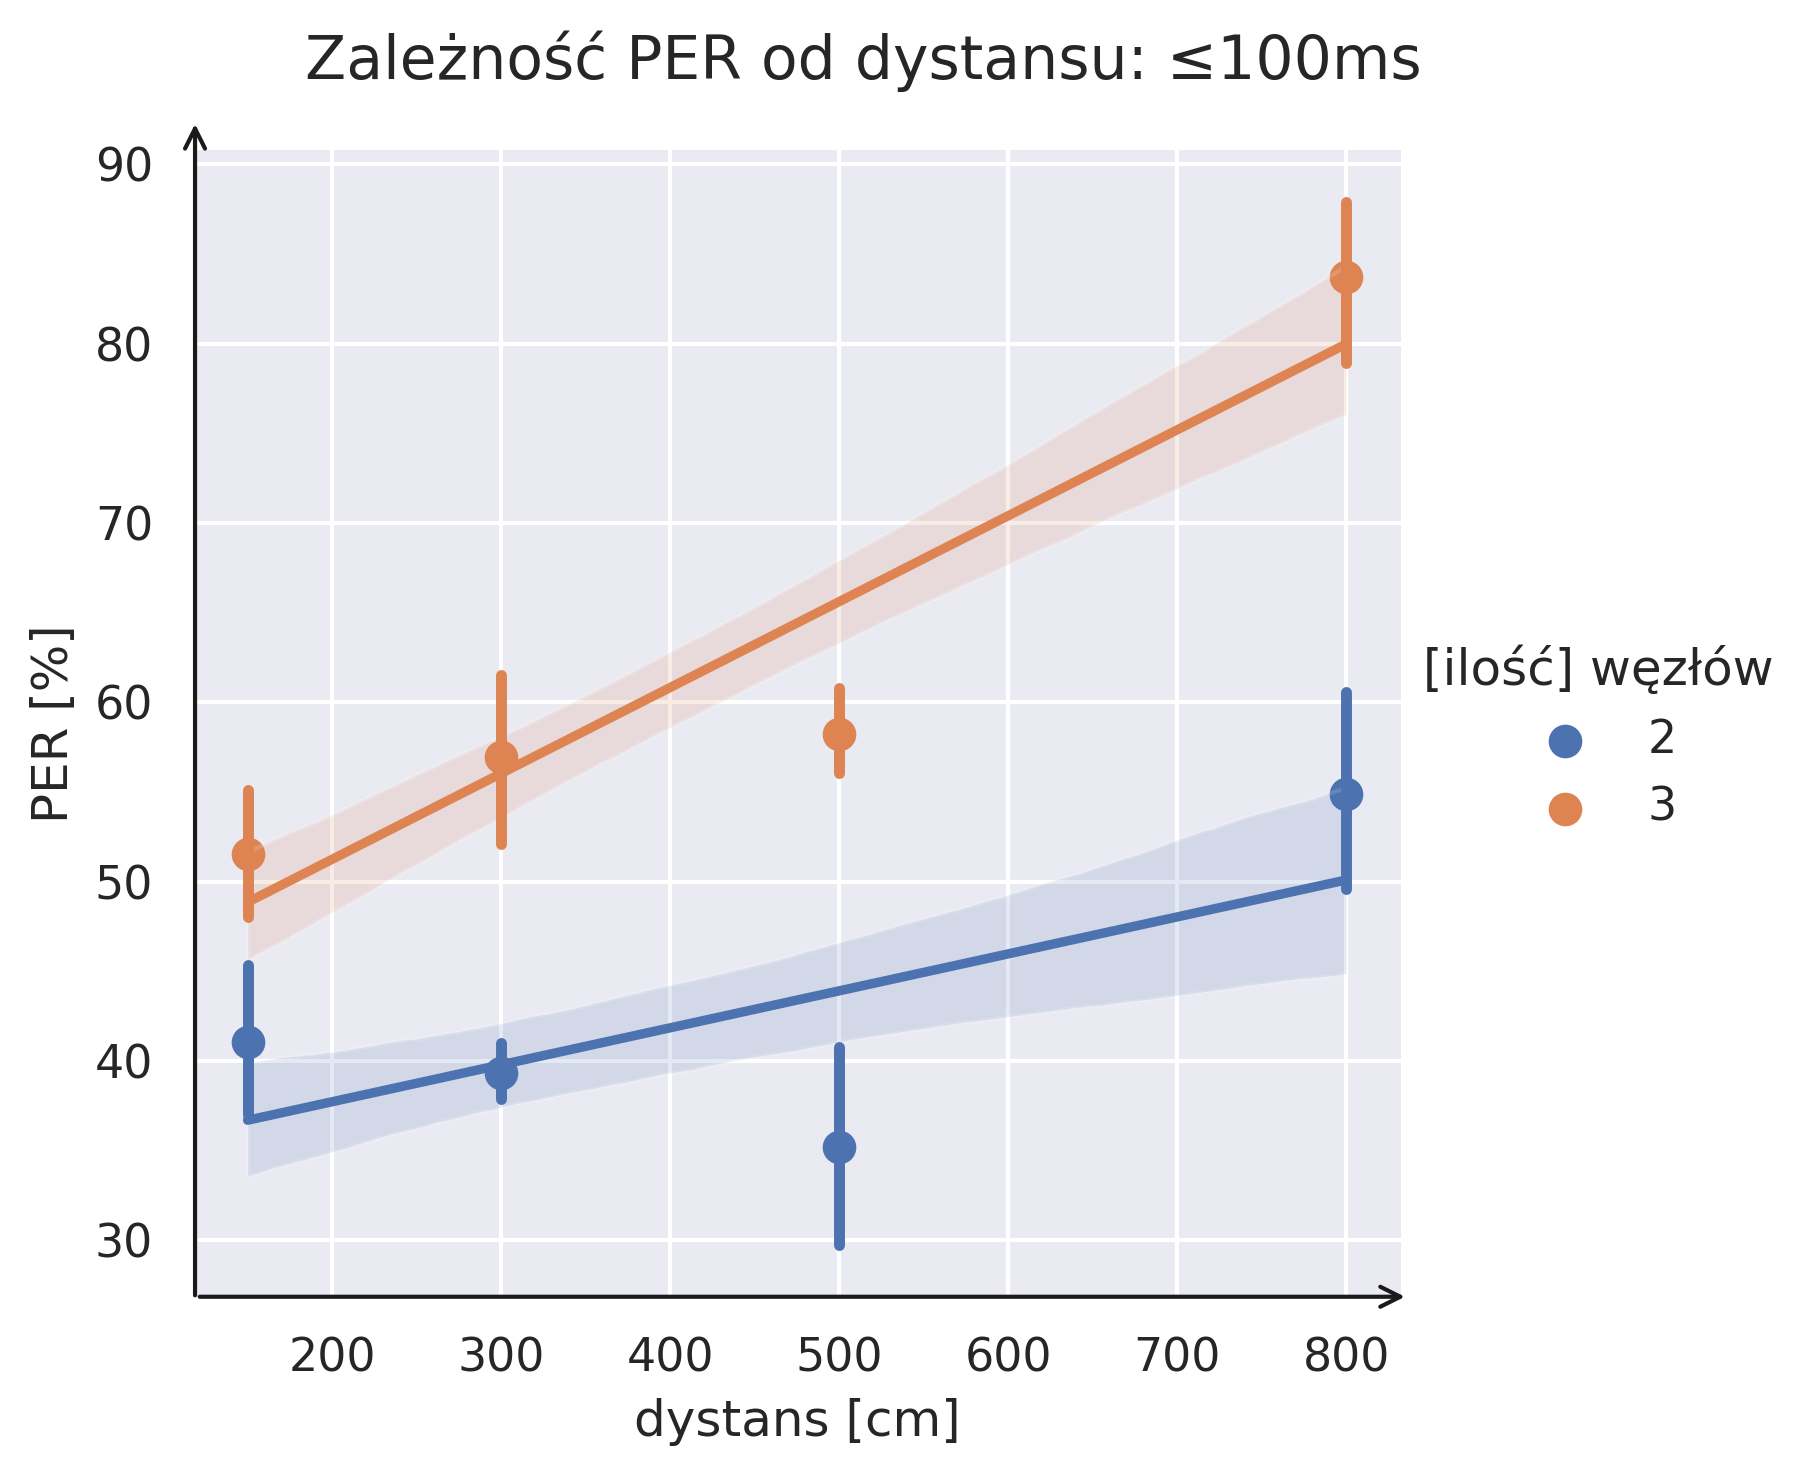
\includegraphics[width=0.618\linewidth]{per_to_distance_under_100ms.png}
	\caption{Zależność PER od dystansu dla zapytań o częstości $\leqslant$ 100ms dla różnej liczby węzłów}
	\label{rys:per_to_distance_under_100ms}
\end{figure}

\begin{figure}[!htb]
	\centering 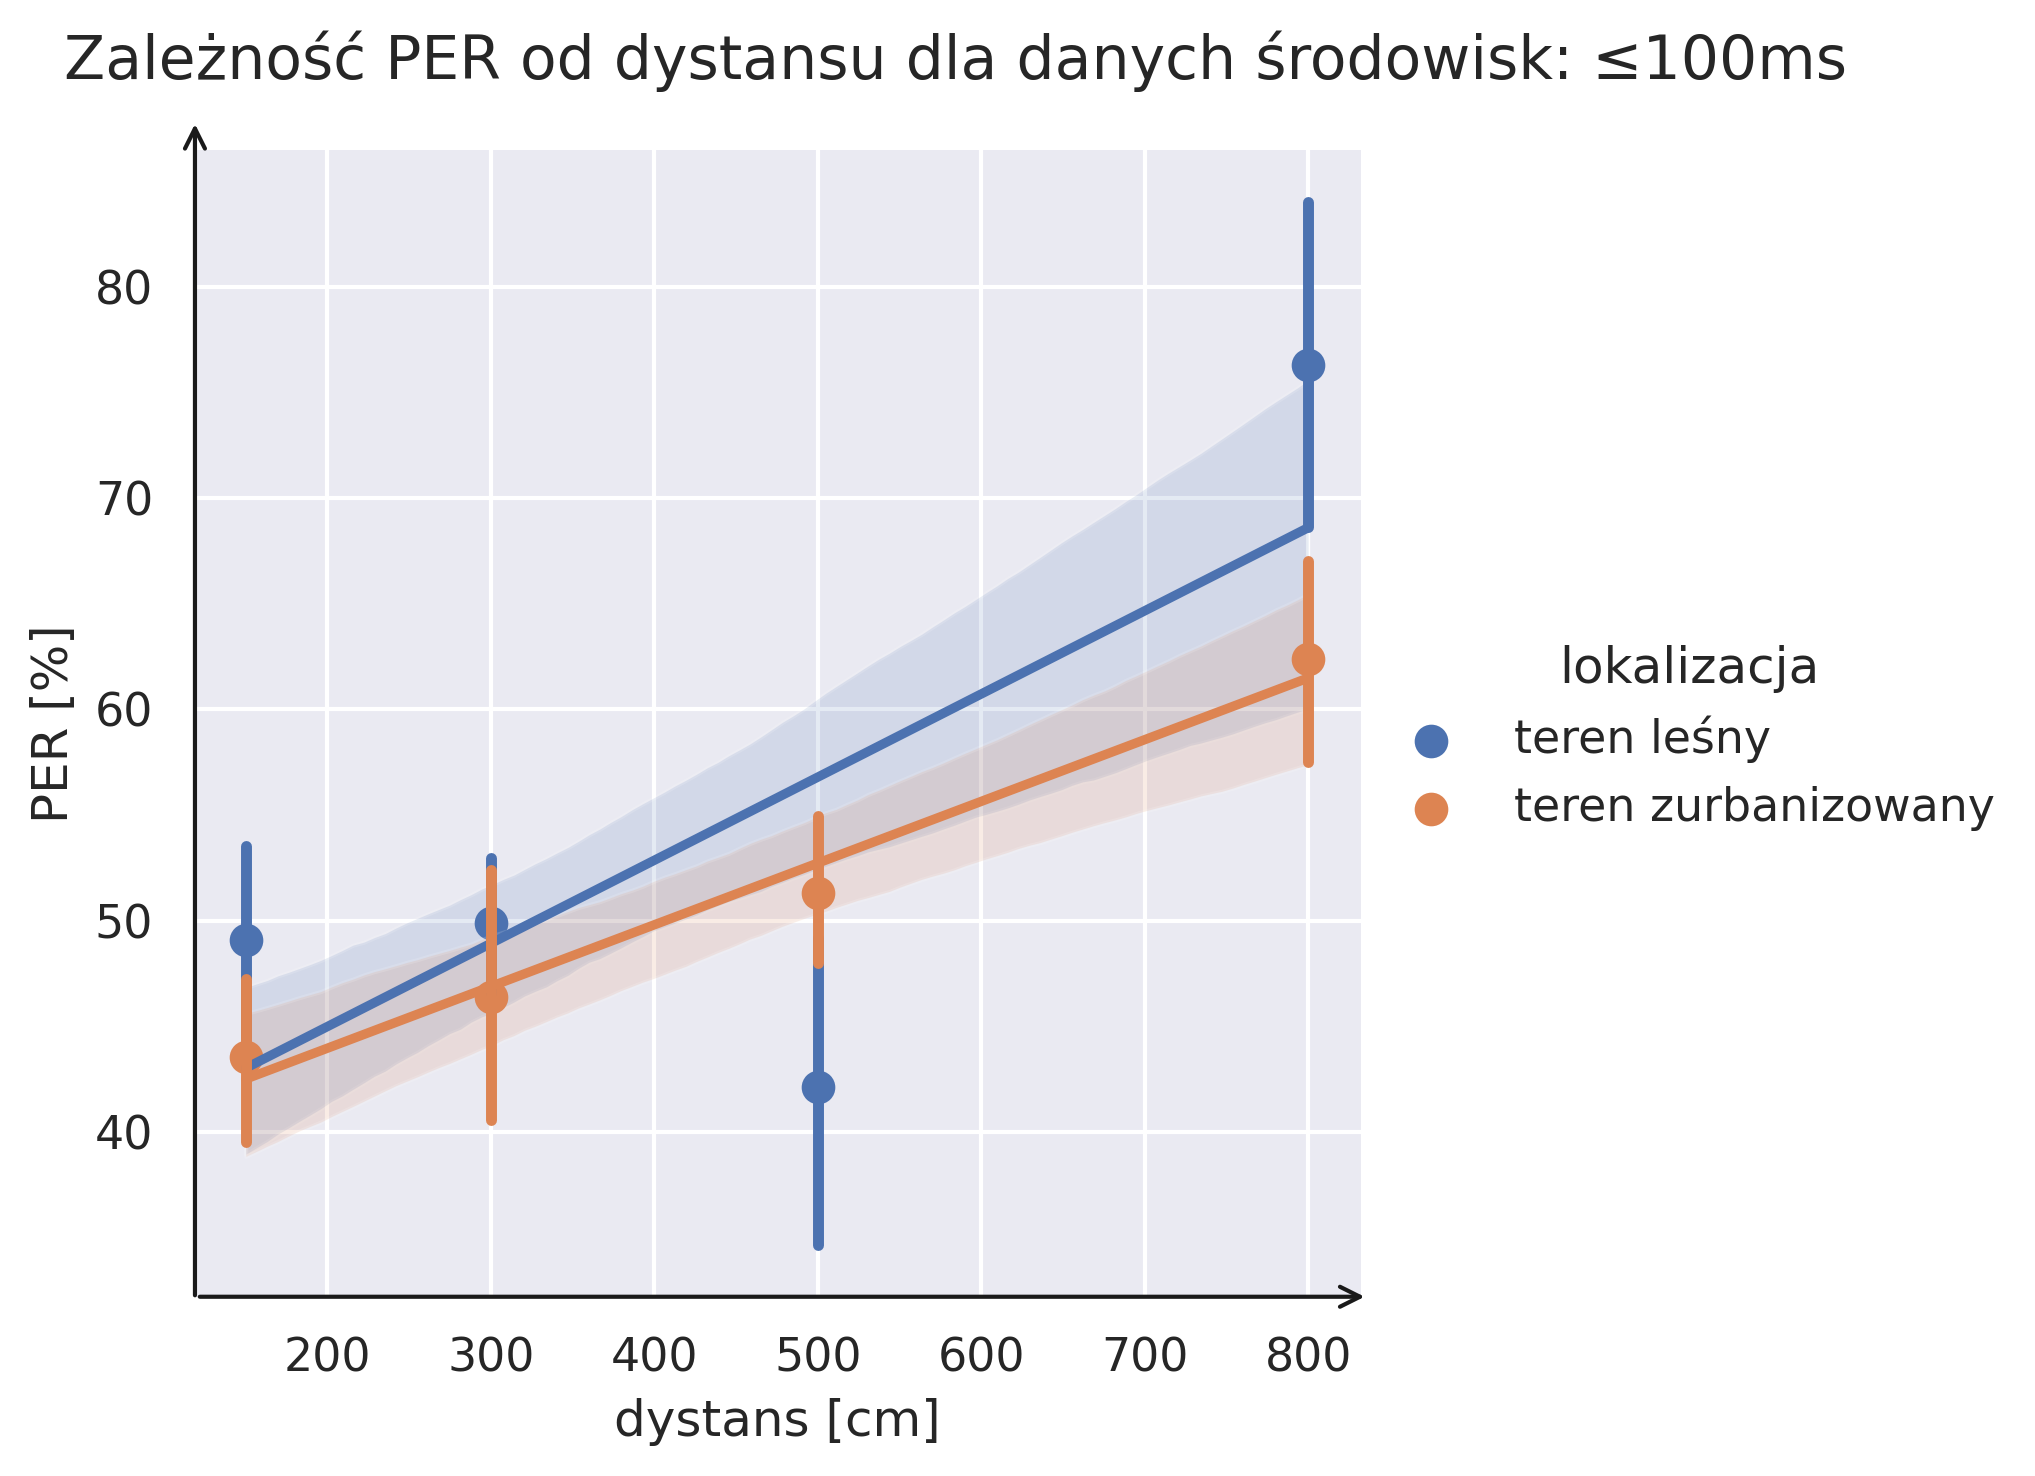
\includegraphics[width=0.618\linewidth]{per_to_distance_under_100ms_different_envs.png} 
	\caption{Zależność PER od dystansu dla zapytań o częstości $\leqslant$ 100ms w wybranych środowiskach bez rozróżnienia na liczbę węzłów}
	\label{rys:per_to_distance_under_100ms_different_envs}
\end{figure}

\begin{figure}[!htb]
	\centering 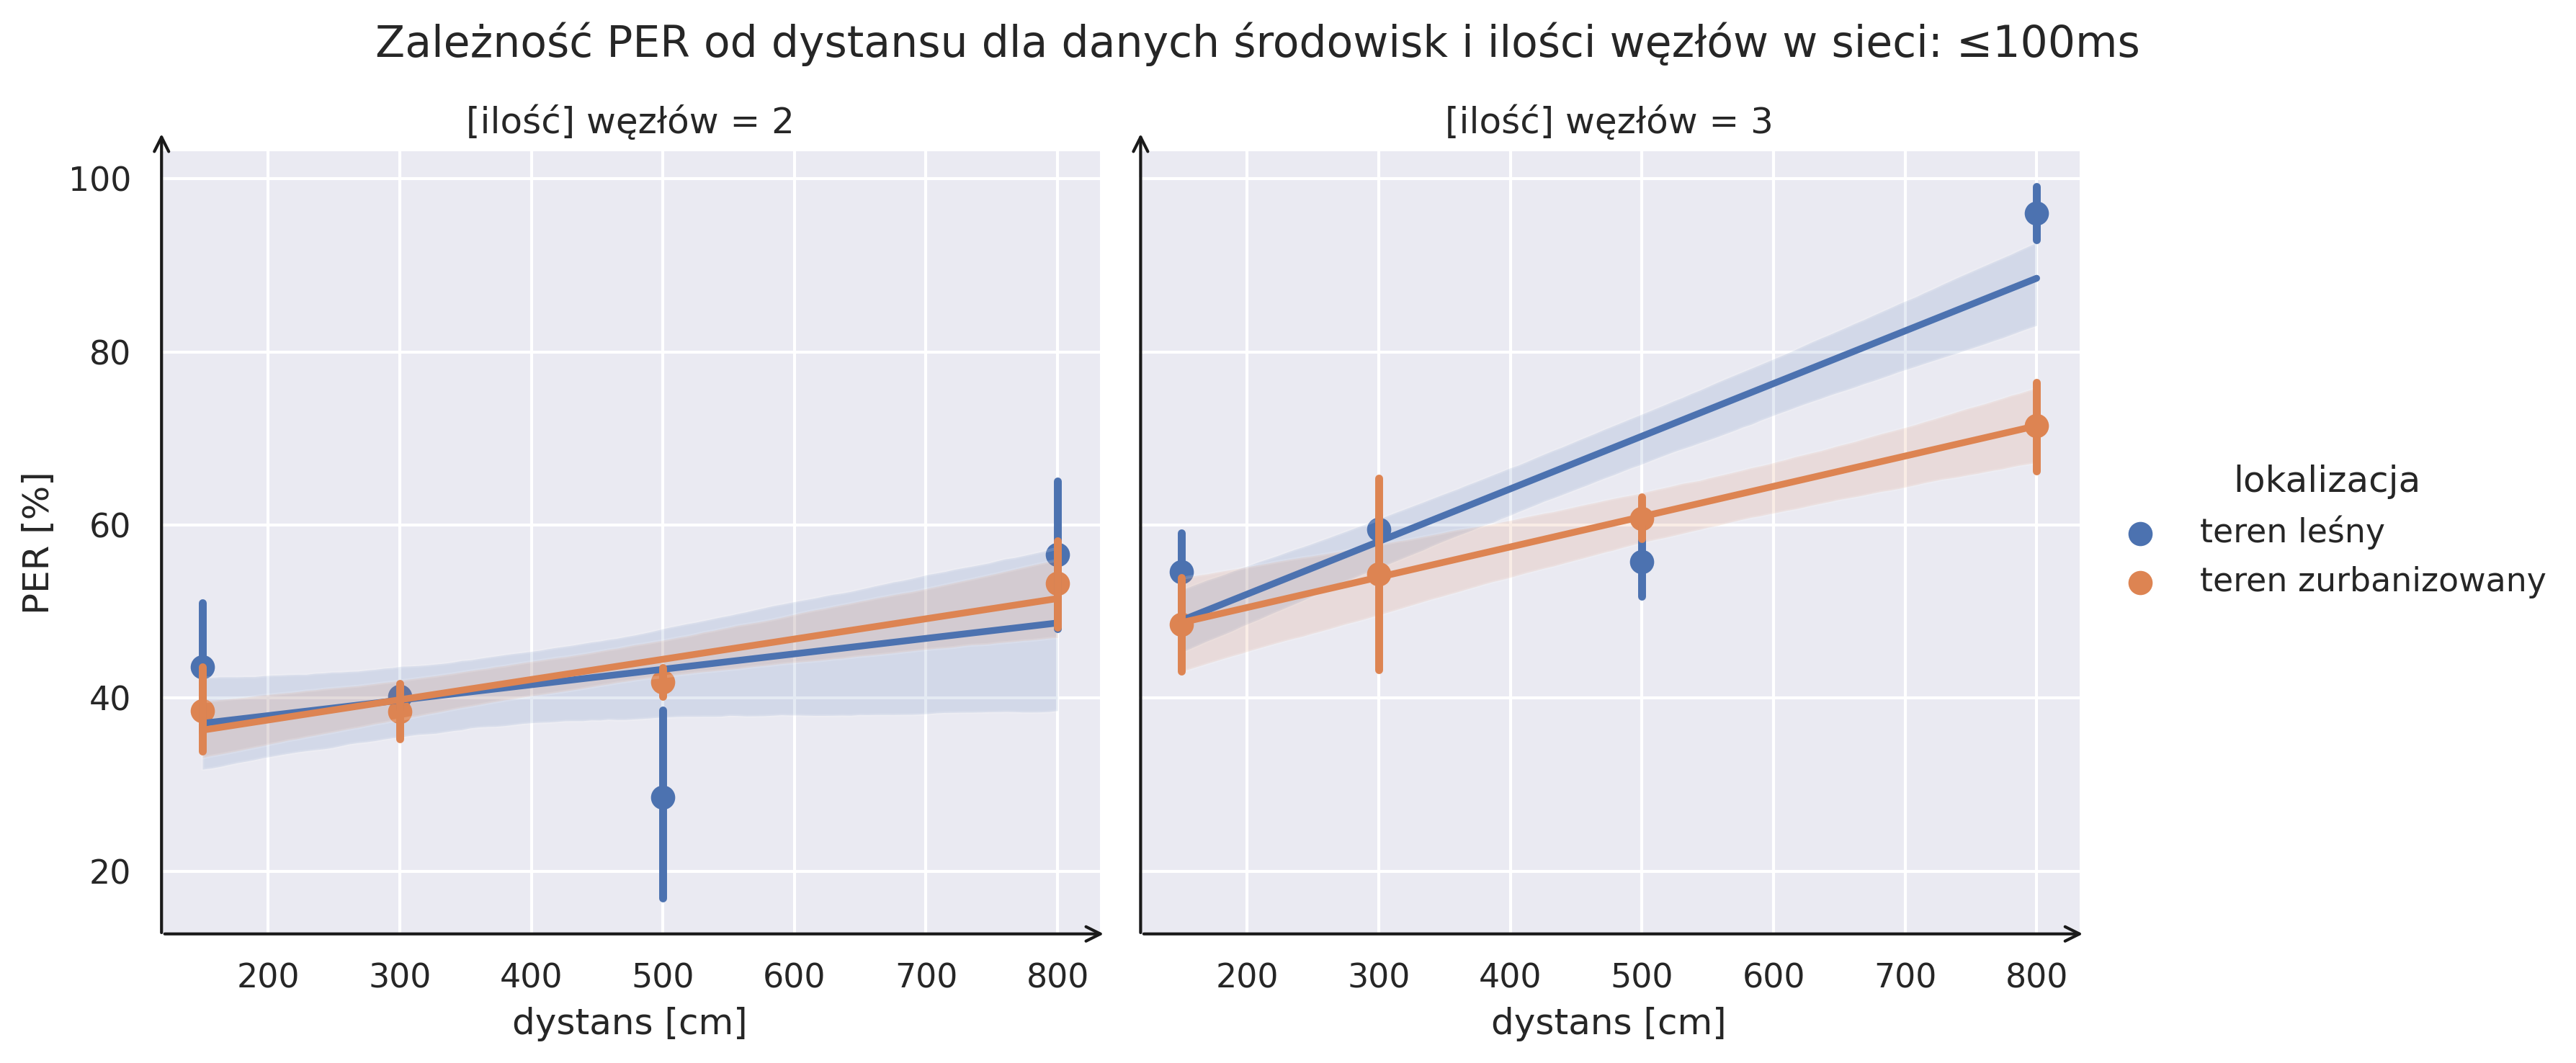
\includegraphics[width=0.99\linewidth]{per_to_distance_under_100ms_different_envs_and_nodes.png}
	\caption{Zależność PER od dystansu dla zapytań o częstości $\leqslant$ 100ms w wybranych środowiskach i liczbę badanych węzłów}
	\label{rys:per_to_distance_under_100ms_different_envs_and_nodes}
\end{figure}

\begin{figure}[!htb]
	\centering 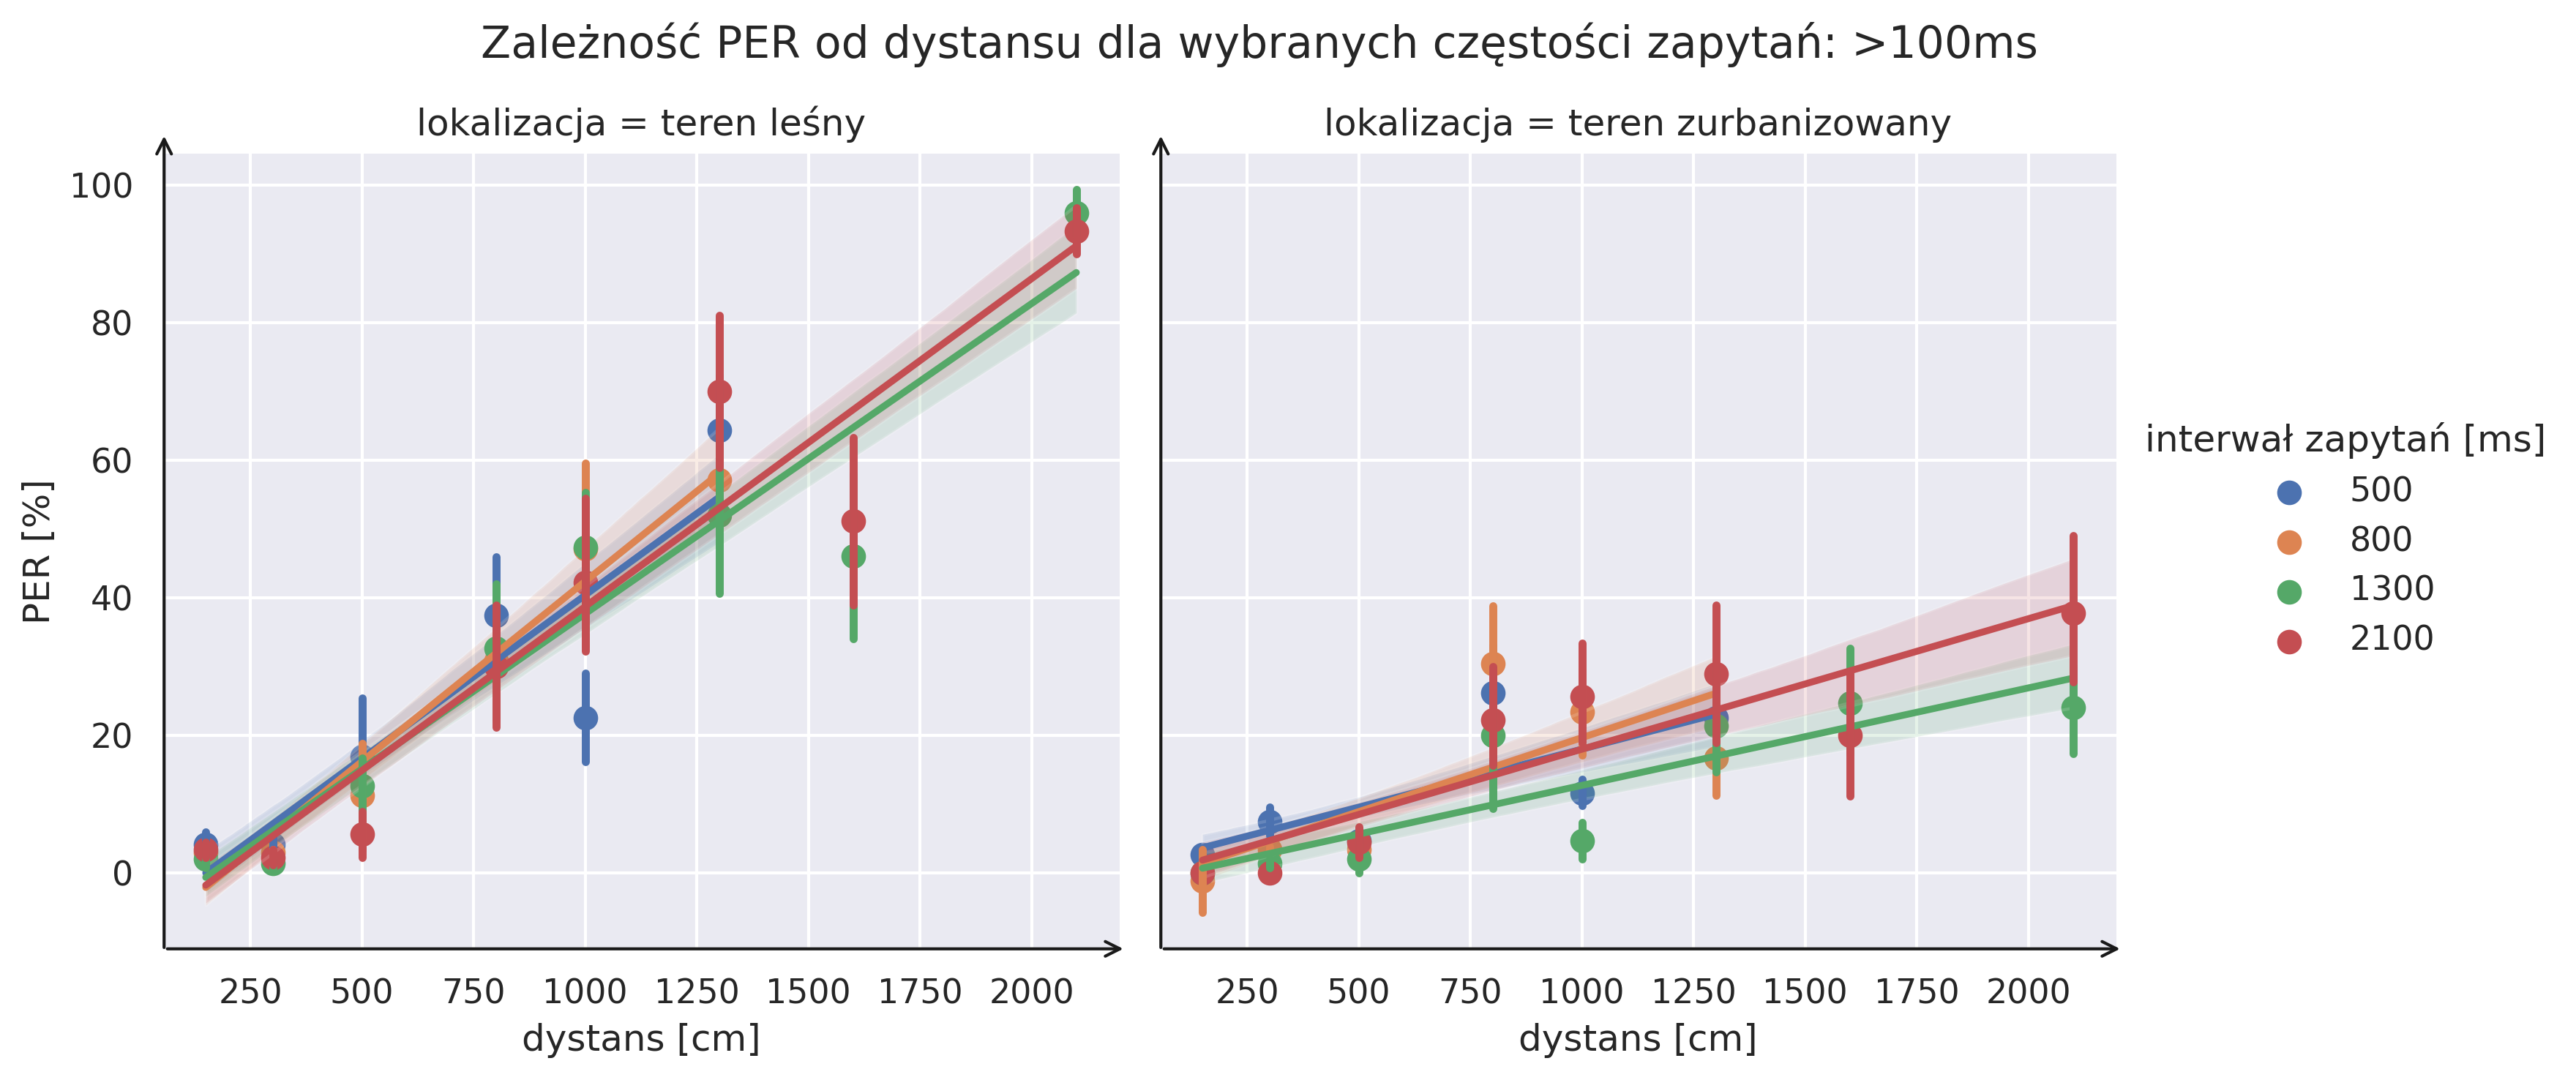
\includegraphics[width=0.99\linewidth]{per_to_distance_over_100ms_different_envs_different_ping_interval.png} 
	\caption{Zależność PER od dystansu dla zapytań o częstości >100ms w wybranych środowiskach}
	\label{rys:per_to_distance_over_100ms_different_envs_different_ping_interval}
\end{figure}


%%%%%%%%%%%%%%%%%%%%%%%%%%%%%%%%%%%%%%%%%%%%%%%%%%%%%%%%%%%%%%%%%%%%%%%%%%%%%%%%
%% SUBSECTION: Zależność PER względem odległości między węzłami
%%%%%%%%%%%%%%%%%%%%%%%%%%%%%%%%%%%%%%%%%%%%%%%%%%%%%%%%%%%%%%%%%%%%%%%%%%%%%%%%
\subsection{Zależność PER względem odległości między węzłami}

\begin{figure}[!htb]
	\centering 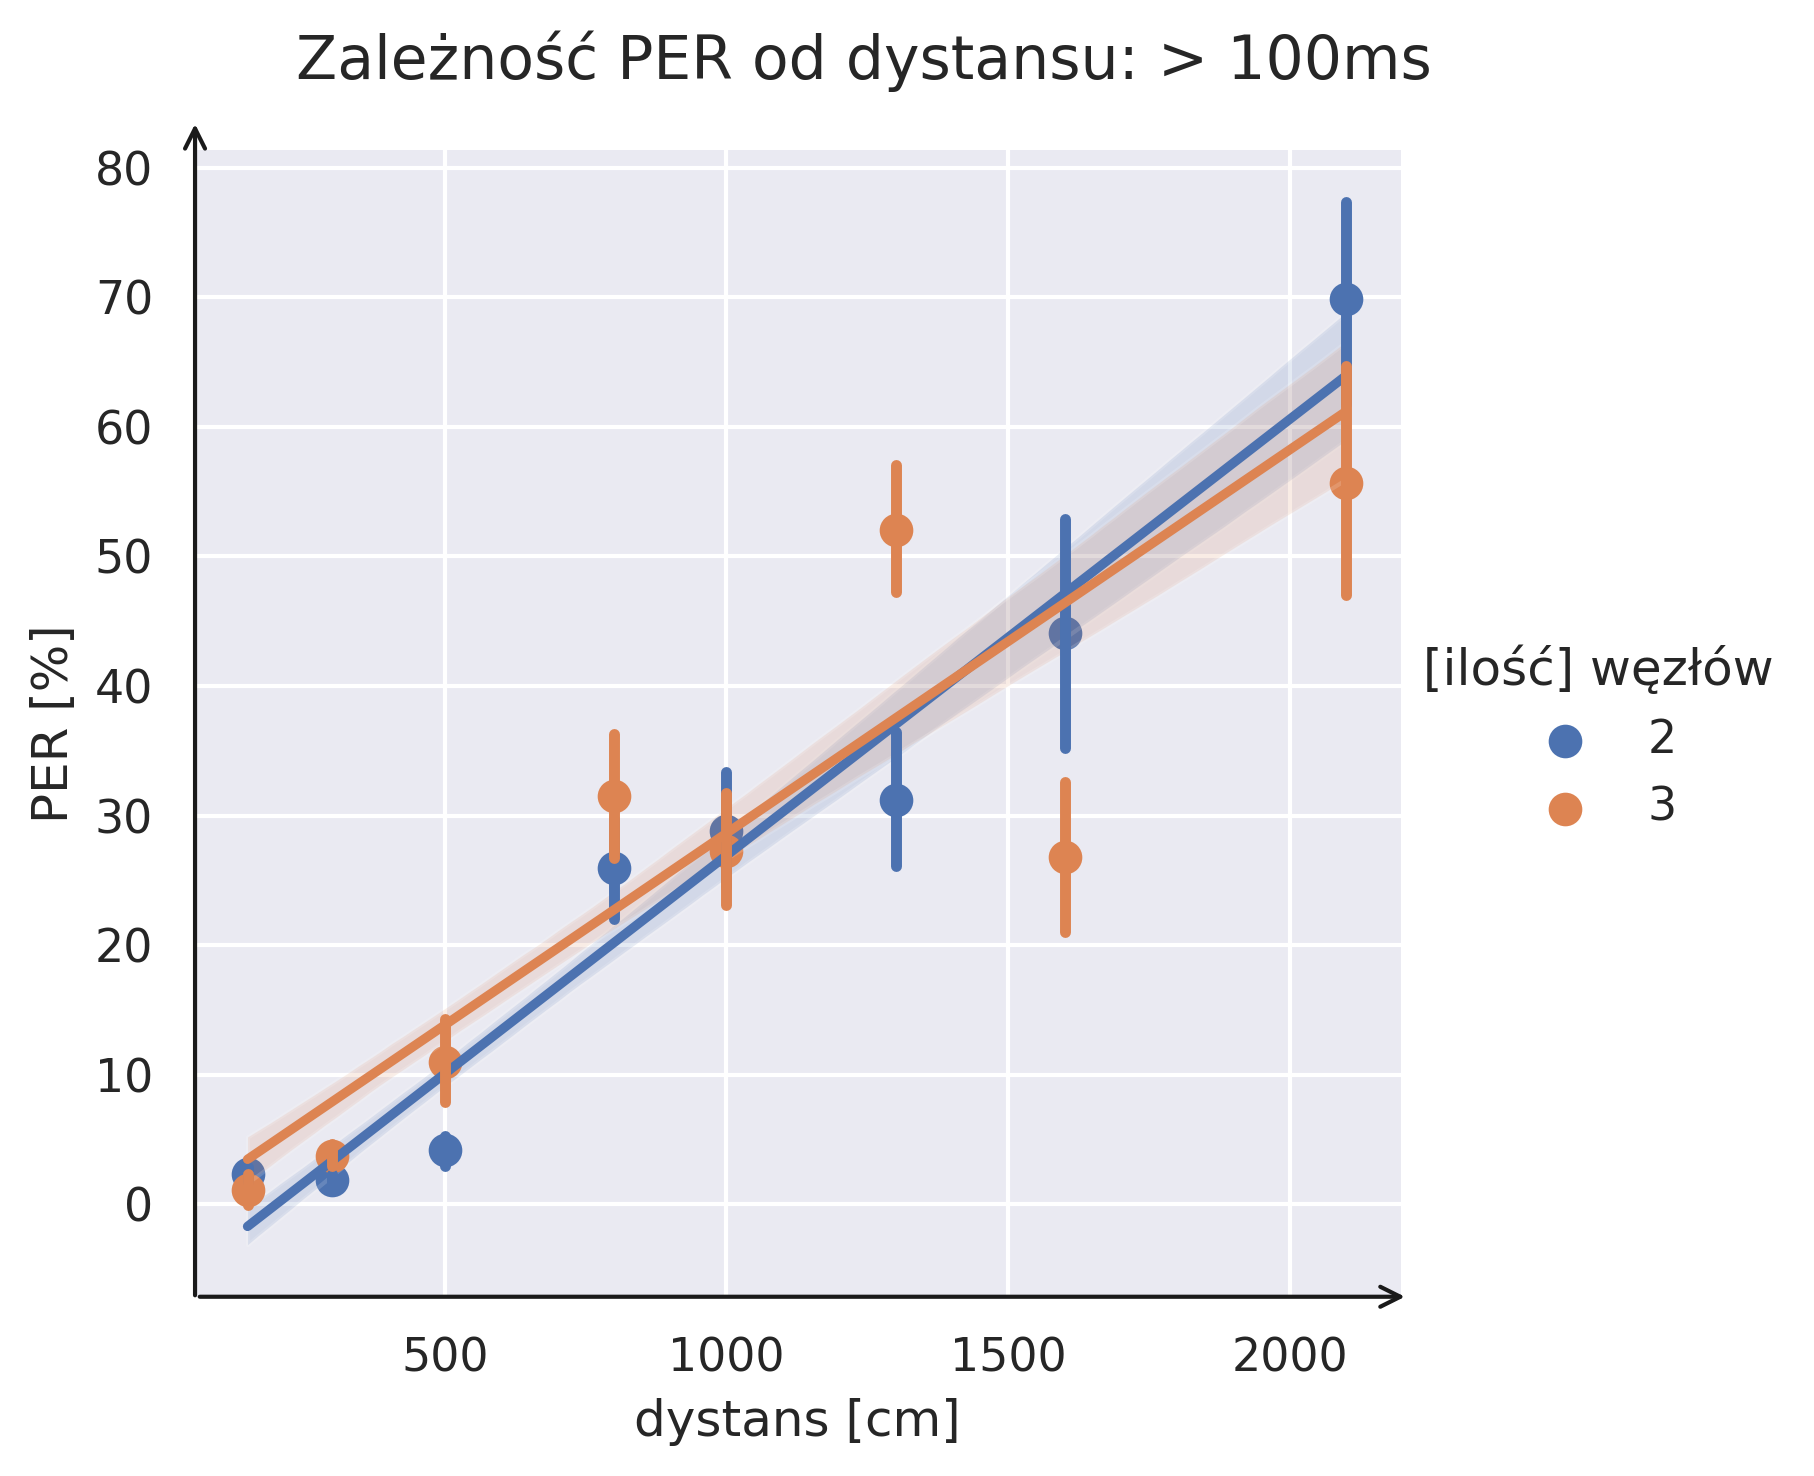
\includegraphics[width=0.618\linewidth]{per_to_distance_over_100ms.png}
	\caption{Zależność PER od dystansu dla zapytań o częstości >100ms dla różnej liczby węzłów}
	\label{rys:per_to_distance_over_100ms}
\end{figure}

\begin{figure}[!htb]
	\centering 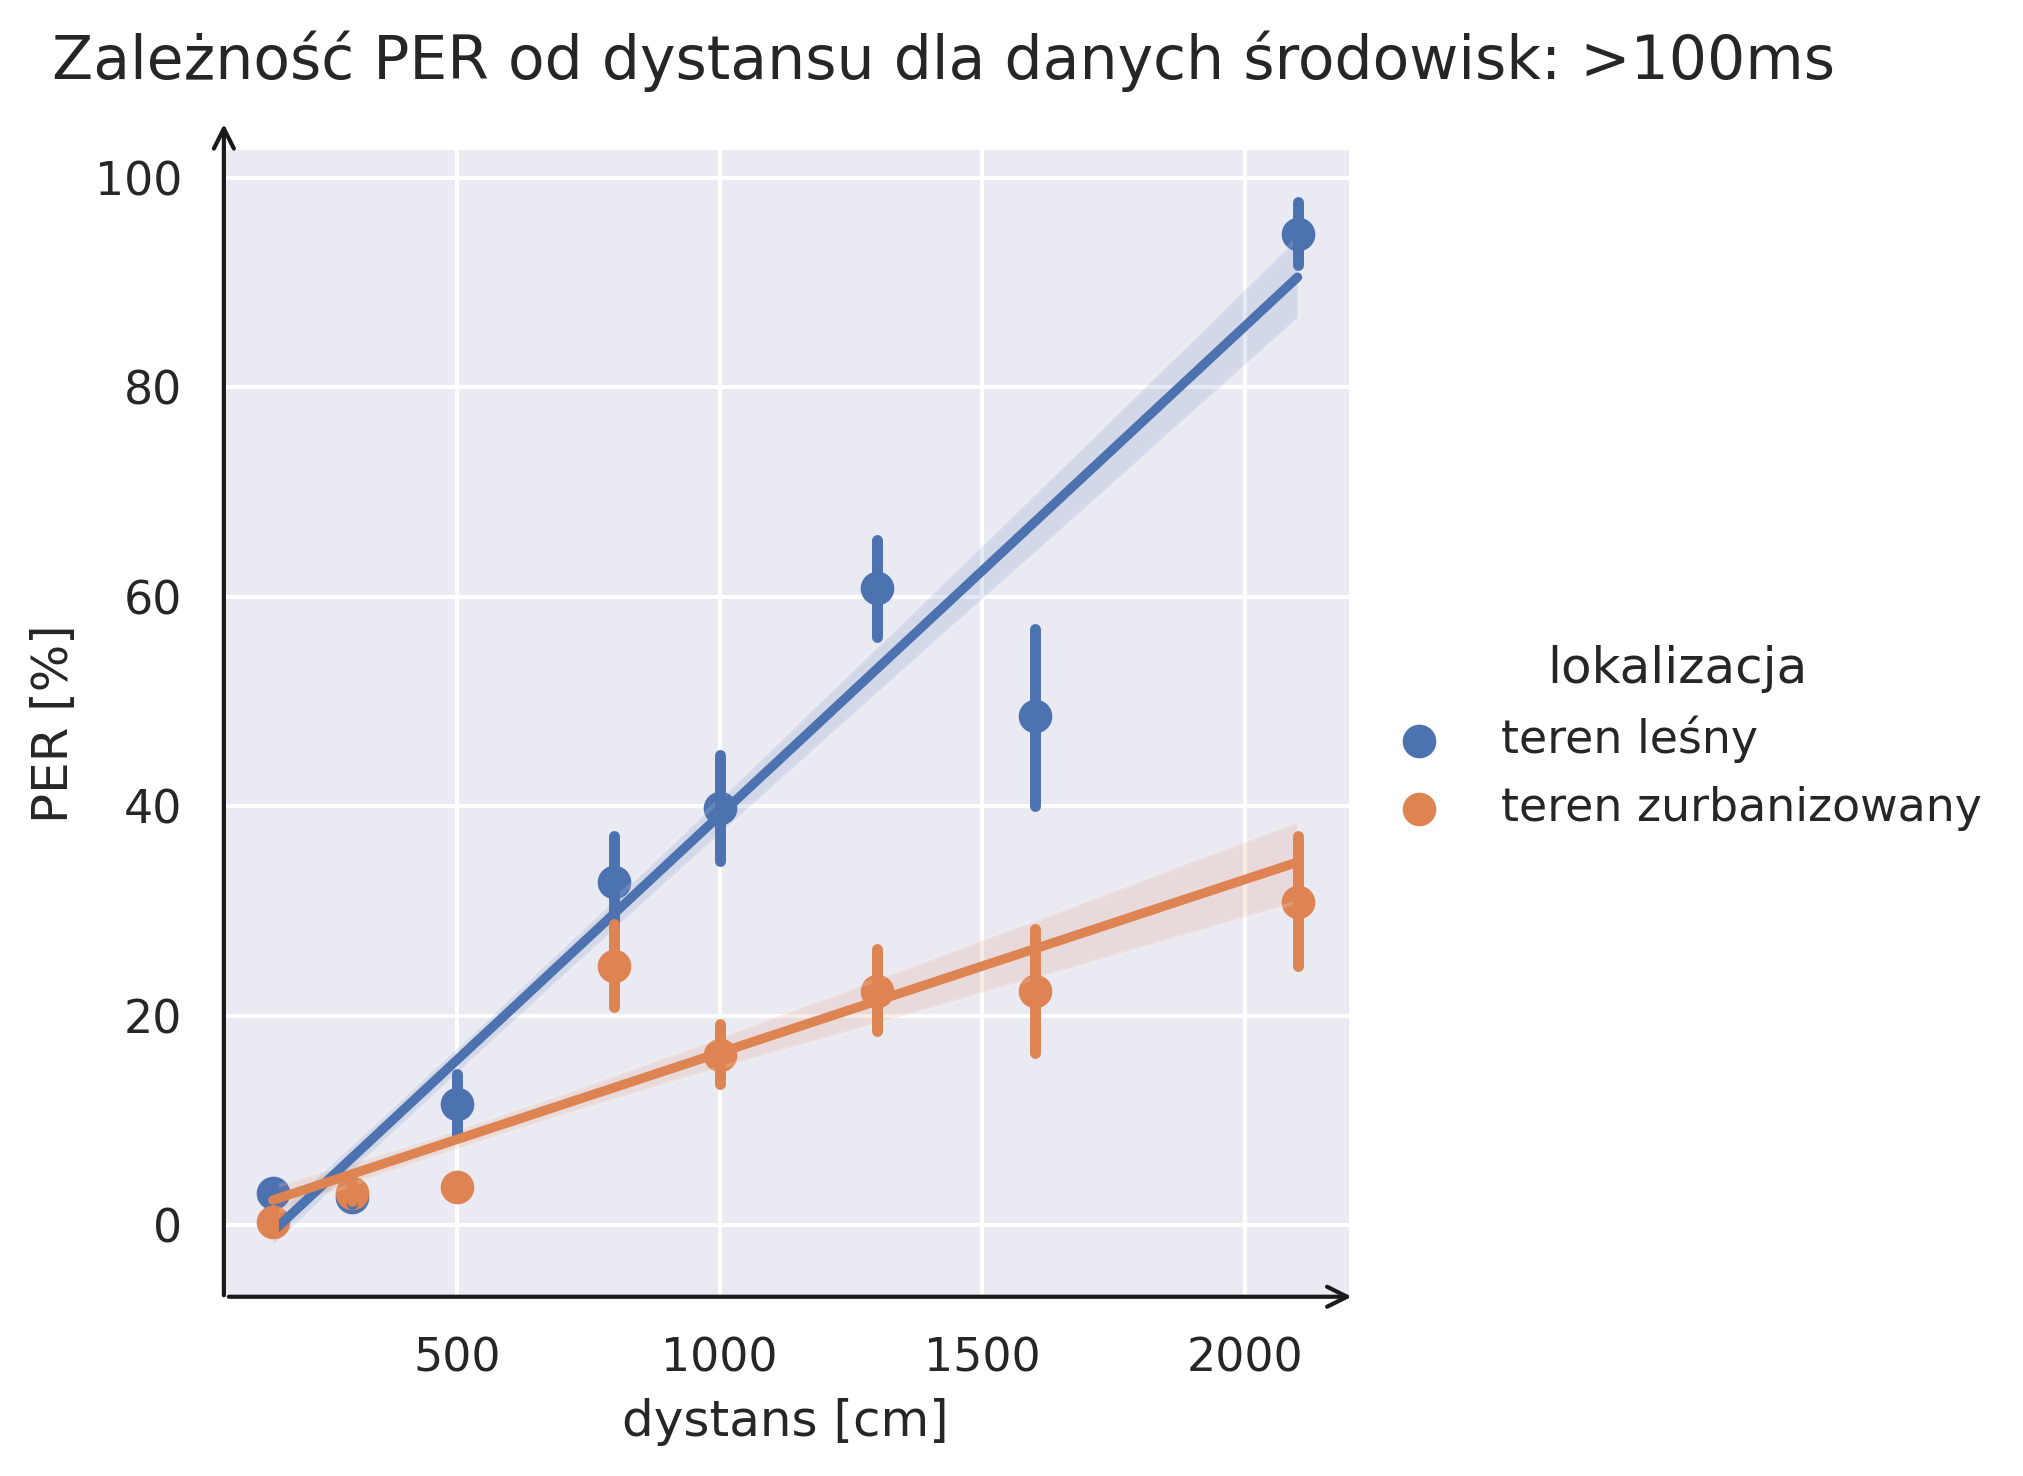
\includegraphics[width=0.618\linewidth]{per_to_distance_over_100ms_different_envs.png} 
	\caption{Zależność PER od dystansu dla zapytań o częstości >100ms w wybranych środowiskach bez rozróżnienia na liczbę węzłów}
	\label{rys:per_to_distance_over_100ms_different_envs}
\end{figure}

\begin{figure}[!htb]
	\centering 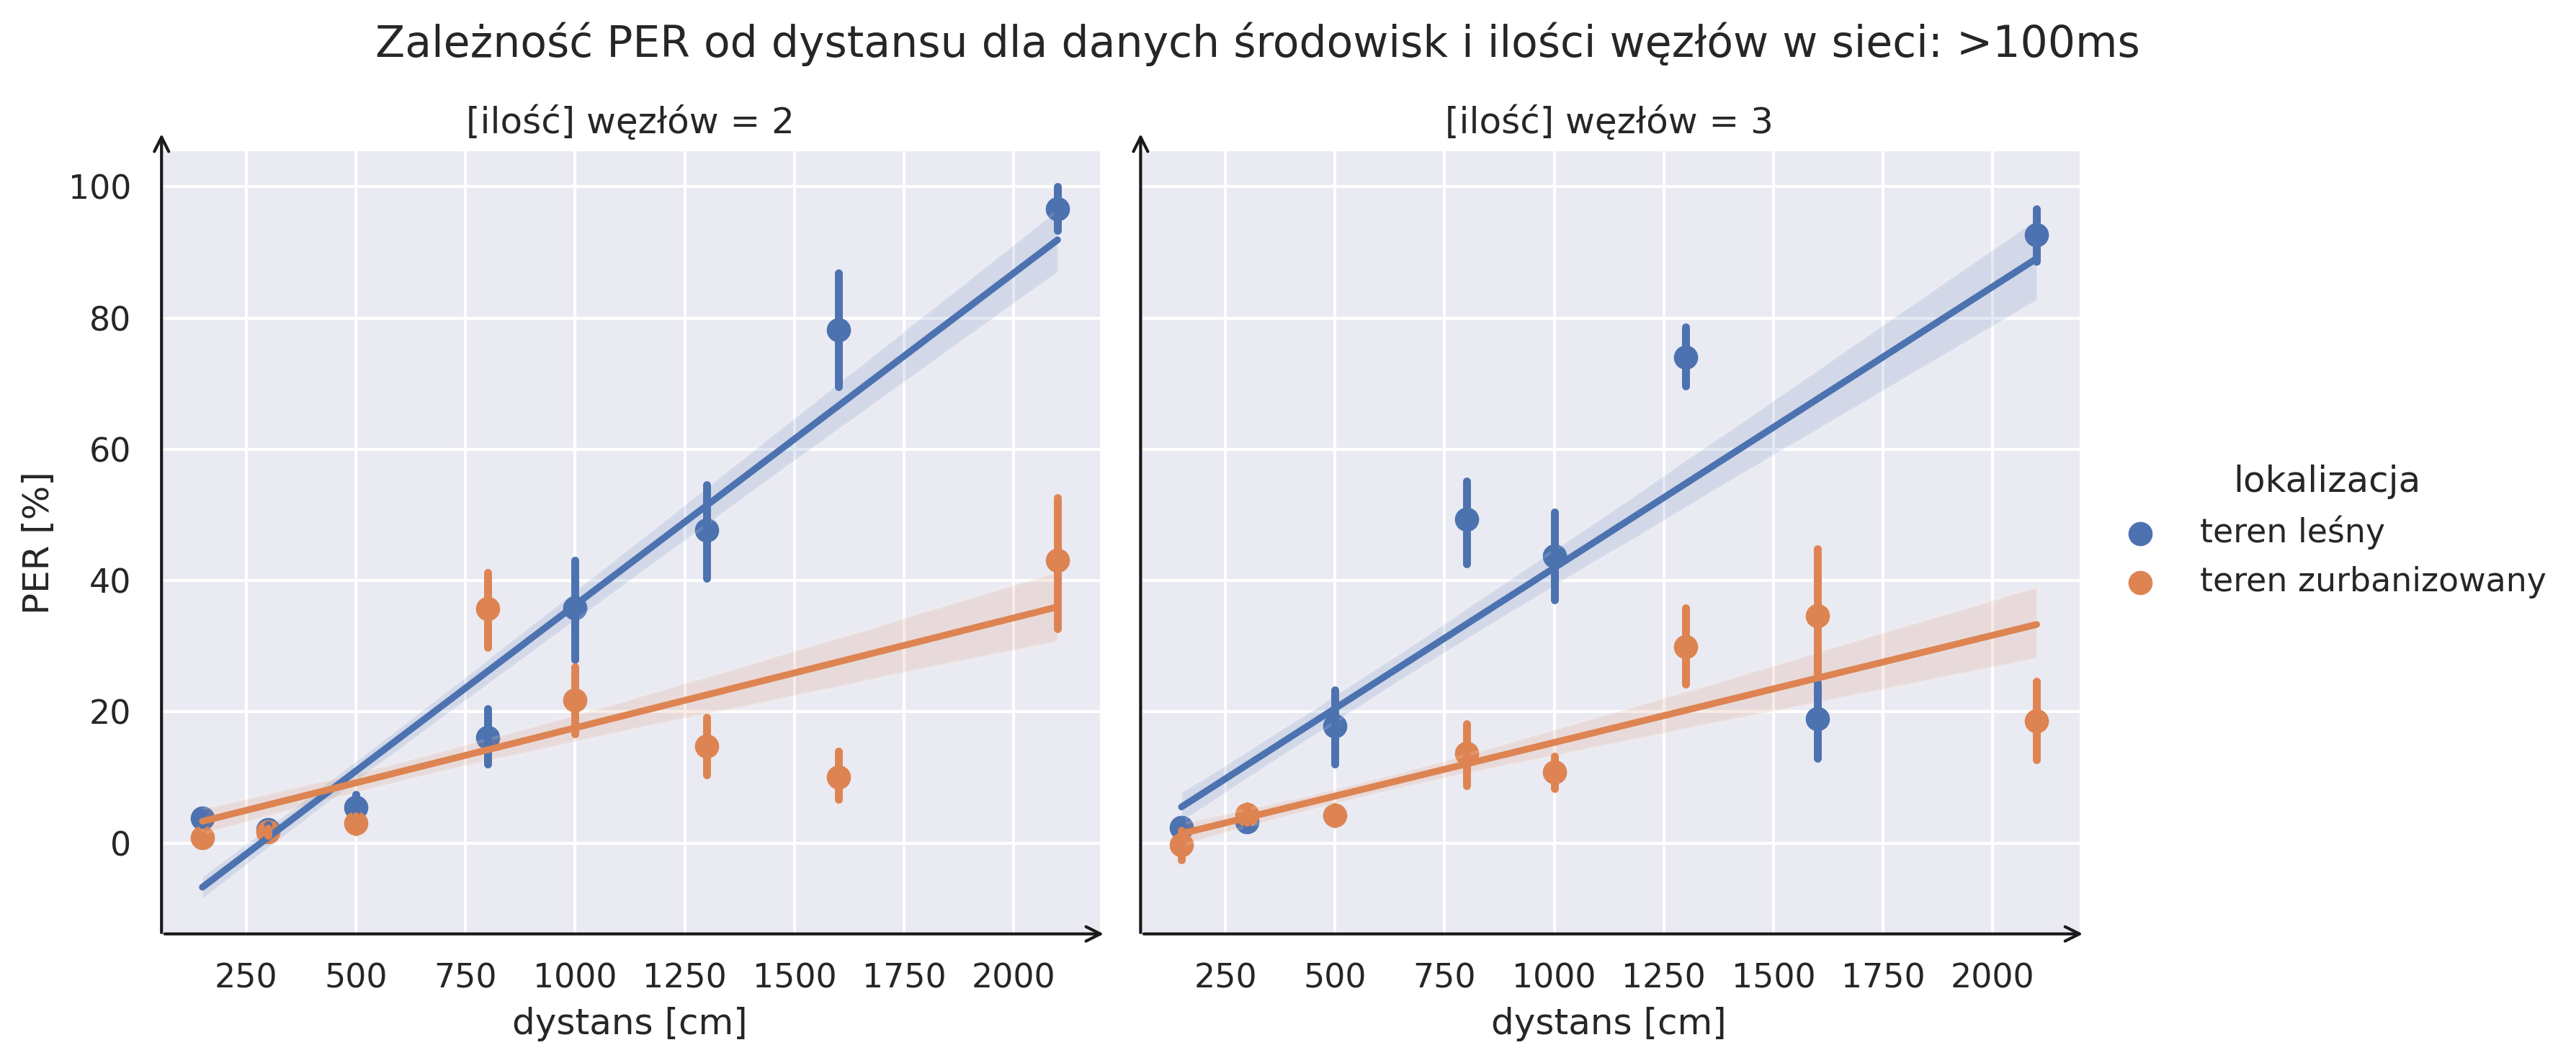
\includegraphics[width=0.99\linewidth]{per_to_distance_over_100ms_different_envs_and_nodes.png}
	\caption{Zależność PER od dystansu dla zapytań o częstości >100ms w wybranych środowiskach i liczbę badanych węzłów}
	\label{rys:per_to_distance_over_100ms_different_envs_and_nodes}
\end{figure}

